\documentclass[oneside,abstractoff,a4paper]{scrartcl}

\usepackage{amsmath, amssymb, xspace}
\DeclareMathOperator*{\argmax}{arg\,max}
\usepackage{array}
\usepackage{multirow}
\usepackage{epsfig}
%\usepackage{ngerman}
\usepackage{german}
\usepackage[latin1]{inputenc}
\usepackage{t1enc}
\usepackage{graphicx}
\usepackage{amstext}
\usepackage{hyperref}
\usepackage{wrapfig}
\usepackage{scrpage2}
\usepackage{bibgerm}
\usepackage[ngerman]{cleveref}
\usepackage[shortcuts,nogroupskip,acronym]{glossaries}
\usepackage[binary-units=true]{siunitx}
\usepackage{tikz}
\usetikzlibrary{shapes,arrows,positioning,calc}
\usepackage{pgfplots}
\pgfplotsset{compat=1.14}
\usepackage{selinput}
\SelectInputMappings{
	adieresis={ä},
	germandbls={ß},
	Euro={€},
}
\usepackage{subfig}
\bibliographystyle{ieeetr}
\usepackage[section]{placeins}

\subject{Softwareprojektpraktikum Lego Mindstorms \\
	Informatik 11 Embedded Software}
\title{Abschlussbericht Team 2
%\\[20mm]
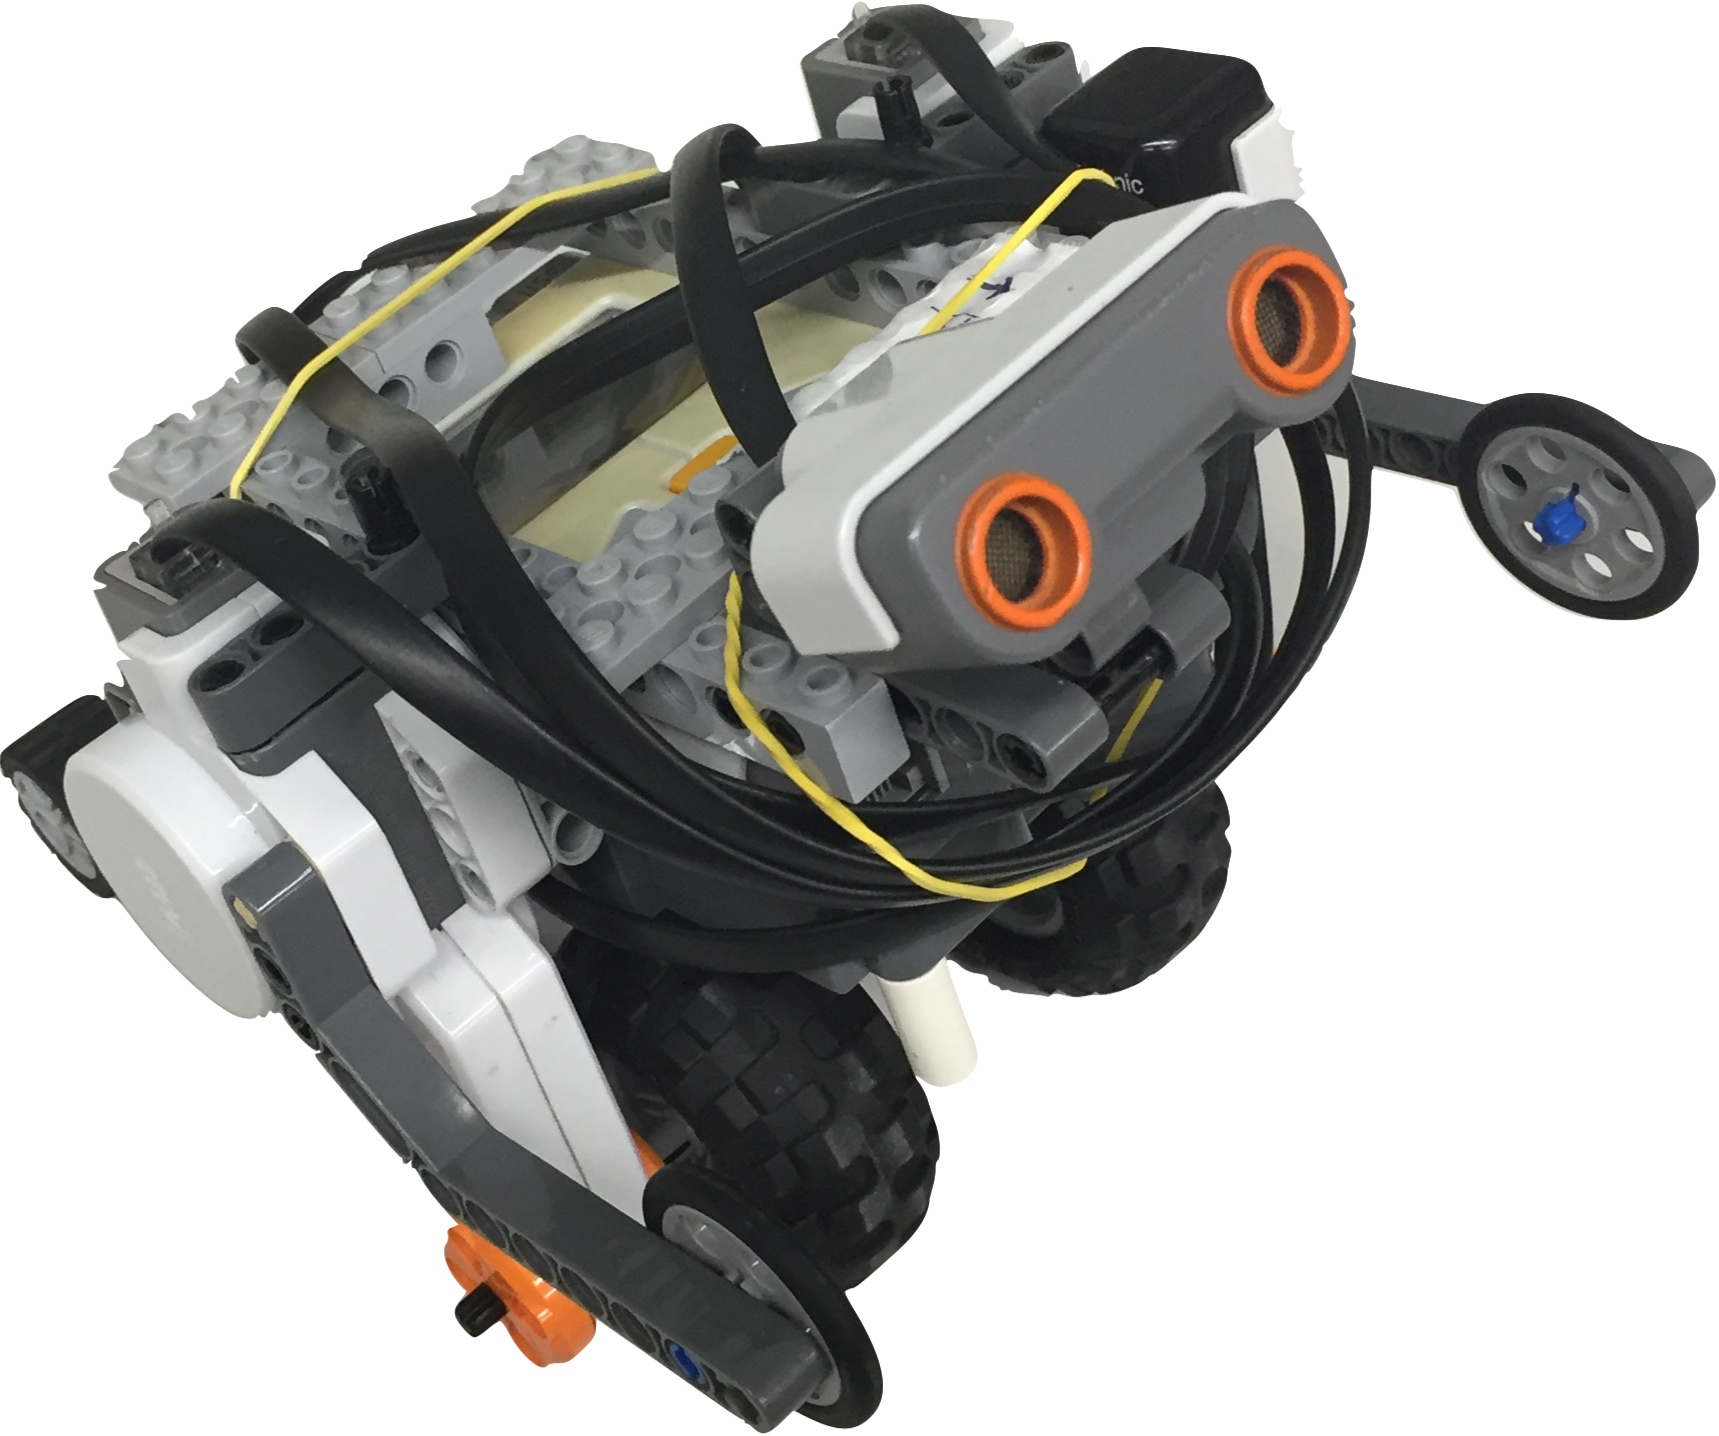
\includegraphics[angle=330,width=\textwidth,height=0.4\textheight,keepaspectratio]{NXT_3.jpg}}

\author{J. Breyer, F. Friedrichs, C. Kloos, G. Kobsik, R. Kupper}
%\publishers{Informatik 11 Embedded Software}
\date{\today}


\newacronym{jvm}{JVM}{Java Virtual Machine}
\newacronym{jre}{JRE}{Java Runtime Environment}
\newacronym{javame}{Java ME}{Java Platform, Micro Edition}
\newglossaryentry{lejos}{
	name=LeJOS,
	description={LeJOS}
}

\begin{document}

\pagestyle{useheadings}
\pagenumbering{roman}
\maketitle
\newpage
\tableofcontents
%\listoffigures
%\listoftables
\cleardoublepage
\pagestyle{scrheadings}
\pagenumbering{arabic}

%\begin{abstract}
%\noindent Abstract
%\end{abstract}

\section{Einleitung}

Im Rahmen des Praktikums \textit{Entwicklung NXT-gesteuerter LEGO-Fahrzeuge mit Java} stand unser Team vor der Aufgabe, aus dem \textit{Lego Mindstorm NXT 1.0} Set einen Segway zu bauen und diesen über das \textit{LeJOS} Betriebssystem mit Java funktionsfähig zu machen. Dabei sollte in diesem Projekt die Softwareentwicklung mit Scrum angewendet werden.
Das Praktikum bestand dabei aus einer Reihe von Abnahmen und Zwischenvorträgen, um den aktuellen Stand des Projekts zu überprüfen. 

Zu Beginn beschäftigte sich das Projekt mit der Einrichtung und Installation von Eclipse und Git, welche die vorgegebenen Werkzeuge für dieses Praktikum darstellen. Als erste große Aufgabe folgte die Implementierung eines PID Reglers, sodass der Segway balancieren kann. Anschließend wurde eine Anforderungsanalyse durchgeführt, die den restlichen Ablauf des Projekts bestimmte. Die nächste Aufgabe stellte schließlich die Entwicklung eines großen zusammenhängenden Systems dar, bestehend aus einer GUI am PC, dem NXT und der Kommunikation zwischen beiden Geräten. Es folgte die Implementierung der Bewegungssteuerung sowie zwei Extras, welche diese Arbeit abschließen sollen. 

Dabei ging es nicht nur um das Programmieren, sondern auch um die Organisation innerhalb eines Teams. Der folgende Bericht dokumentiert die Durchführung und das Ergebnis unserer Gruppe in diesem Projekt.

\section{Anforderungen}

\subsection{Hardware}
\label{subsec:hardware}
Hier betrachten wir die uns zur Verfügung gestellte Hardware, insbesondere die Sensorik des NXT-Bricks.
%glaube da fehlt ein "e"
Der Lego Mindstorms NXT verf"ugt "uber einen \SI{48}{\mega\hertz} ARM-Prozessor, \SI{64}{\kibi\byte} Hauptspeicher sowie \SI{256}{\kibi\byte} Flash-Speicher für Programme.

Der Gyro-Sensor ist ein Einachsen-Gyroskop mit einer Aufl"osung von \SI{1}{\degree\per\second}. Bedingt durch die Diskretisierung werden Winkelgeschwindigkeiten unter \SI{1}{\degree\per\second} nicht erkannt. Folglich l"asst sich durch aufsummieren der Winkelgeschwindigkeiten kein absoluter Winkel berechnen. Eigene Tests ergaben einen Fehler von bis zu \SI{15}{\degree} pro Umdrehung, trotz regelmäßiger Rekalibrierung.

Für die Ansteuerung der Räder stehen zwei Motoren zur verfügen. Die Motoren selbst verfügen über einen Quadraturencoder mit einer Auflösung von \SI{720}{Ticks} pro Umdrehung. Softwareseitig wird allerdings nur eine Auflösung von \SI{360}{Ticks} pro Umdrehung bereitgestellt.

Der Ultraschall-Sensor erkennt Objekte innerhalb eines Kegels mit \SI{30}{\degree} Öffnungswinkel. Die Distanzauflösung betragt \SI{1}{\centi\meter}. Der theoretische Bereich in welchem Objekte erkannt werden können ist somit \SI{1}{\centi\meter} bis \SI{254}{\centi\meter}, der tatsächliche Bereich liegt allerdings eher bei \SI{7}{\centi\meter} bis \SI{160}{\centi\meter}~\cite{NXTtime_ussensor}. Durch den Wert 255 wird signalisiert, dass kein Hindernis erkannt wurde. Leider wird durch den selben Wert ebenfalls ein Fehler bei der Distanzbestimmung signalisiert, was die Hinderniserkennung stark erschwert. Bei eignen Tests traten die Fehler sehr häufig auf. Funktionsbedingt können schalldämpfende Oberfläche nur schlecht erkannt werden.

Auf PC-Seite werden eigene Laptops verwendet, so dass dort keine besonderen Einschränkungen vorliegen.
%ist es notwendig die technisches Details der Hardware die wir zur Verfügung haben zu erwähnen? Gute Formatierung
%Ich denke schon, da die Hardware ja maßgeblich die Anforderungen beeinflusst. Das gehört zur Anforderungsanalyse.
\subsection{Software LeJOS}

\ac{lejos} ist eine \ac{jvm} und kann als alternative Firmware für den Lego NXT verwendet werden.
Die \ac{lejos} NXT Runtime stellt eine minimale Standardbibliothek zur Verfügung. Lambda-Ausdrücke werden nicht unterstützt.

Der Scheduler arbeitet strikt nach Priorität und verwendet bei Threads gleicher Priorität Round Robin mit einem Intervall von \SI{2}{\milli\second}.

\subsection{Issues}
Die von der Betreuern gestellten Anforderungen wurden der Einf"uhrungspr"asentation entnommen und in GitLab (vgl. \cref{subsec:addConcepts}) als Issues strukturiert. Hierzu wurde im Zuge eines Meetings ein Brainstorming durchgeführt, um alle Anforderungen zu erfassen und den entsprechenden von der Leitung vorgegebenen Deadlines zuzuordnen. Diese groben Anforderungen wurden danach weiter spezifiziert und in den Issues in kleinere Teilaufgaben aufgeteilt, um den verantwortlichen Programmierern in jeder Woche einen Leitfaden zu bieten. Alle Issues wurden mit Labeln versehen, die unter anderem die Abnahme, zu der die Anforderung erfüllt sein musste, die voraussichtlich beteiligten Programmierer und eine grobe Einteilung in die Software-Komponente (beispielsweise GUI, PID-Regler oder Kommunikation) kennzeichneten. Die derartige Organisation bot den Programmierern eine schnelle "Ubersicht über bevorstehende Aufgaben. Dieses Konzept wurde ab Abnahme 3 umgesetzt.

\subsubsection{Struktur}
Die derart angelegten Issues waren strukturell gleich aufgebaut. Ein Issue bestand aus einer aussagekr"aftigen "Uberschrift, die die zu erf"ullende Anforderung auf den ersten Blick erkennbar machte, sowie einer kurzen Beschreibung der Anforderung. Der erste Unterpunkt Umsetzung beinhaltete die spezifizierte Zusammensetzung der Anforderung und die "Ubereinkunft unserer Gruppe über die Art der Implementierung.

Im optionalen Anwendungsfall wurde eine beispielhafte Durchf"uhrung der Aufgaben angegeben, die einer Erfüllung der jeweiligen Anforderung entsprach. Im Unterpunkt Tests wurden ein oder mehrere Tests mit eventuellen Vor- und Nachbedingungen angegeben, deren Erf"ullung einer Erf"ullung der jeweiligen Anforderung entsprach. Zus"atzlich wurde jedes Issue mit einer Deadline und dem grob gesch"atzten Arbeitsaufwand versehen.

Die derart erfassten Anforderungen wurden von der Projektleitung "uberpr"uft und best"atigt.

\subsubsection{Anforderungen}

\noindent\textbf{Abnahme 1}

F"ur die erste Abnahme wurde eine erfolgreiche Installation der vorgegebenen Entwicklungsumgebung vorgenommen. Zus"atzlich dazu arbeiteten sich die Beteiligten eigenständig in das verwendete Framework und Git ein. Ein gruppeninternes Wiki zur zentralen Bereitstellung wichtiger Informationen wie Tutorials und Protokolle wurde angelegt.

Die Anforderung an die erste Abnahme bestand zudem aus einem ersten Hardware-Konzept und einigen k"urzeren Beispielprogrammen, um das grunds"atzliche Verst"andnis im Umgang mit der Hard- und Software zu demonstrieren. Hierzu wurde ein „Hello World“-Programm, dessen Zweck in der Ausgabe einer einfachen Textzeile auf dem Bildschirm des NXT bestand, ein Programm zur Ansteuerung der einzelnen Motoren sowie eine Kalibrierung und Auslesung des Gyrosensors geschrieben. Zudem befassten sich einzelne Mitglieder bereits mit dem Konzept des Reglers.\\

\noindent\textbf{Abnahme 2}

In der zweiten Abnahme war ein erfolgreiches Balancieren mit nicht notwendigerweise selbstgeschriebenem Code gefordert. Zudem sollte der Aufbau des Segways abgeschlossen sein. Die Projektmanagement-Tools, auf die sich die Gruppe geeinigt hat, wurden ebenfalls vorgestellt.\\

\noindent\textbf{Abnahme 3}

Im Zuge der dritten Abnahme wurden die Anforderungen an das Projekt erhoben und strukturiert in Issues im GitLab eingetragen. Daraus resultierend wurde ein Zeitplan erstellt, an dem sich die Beteiligten orientieren konnten. Als Lastenheft dient die Pr"asentation der Projektleitung, als Pflichtenheft gen"ugen die angelegten Issues. Da zur Erf"ullung dieser Anforderungen nicht alle Mitglieder ben"otigt werden, besch"aftigt sich der Rest der Gruppe mit der Optimierung des Reglers.\\

\noindent\textbf{Zwischenvortrag 1}
    
Zu diesem Termin musste neben einer kurzen Pr"asentation des Arbeitsfortschrittes ein erstes Kommunikationsprotokoll entworfen werden. Zur Ausarbeitung dieses Protokolls trafen sich Repr"asentanten jeder Gruppe, um eine gruppen"ubergreifende Kompatibilit"at zu gew"ahrleisten. Die Anforderungen an die Kommunikation wurden dabei im Voraus erhoben und ein Prototyp von uns entworfen, der in weiten Teilen in das endgültige Protokoll übernommen wurde. \\

\noindent\textbf{Abnahme 4}
    
F"ur die vierte Abnahme teilte sich das Team in zwei kleiner Gruppen auf. Die erste Gruppe besch"aftigte sich mit dem Entwurf einer GUI (vgl. \cref{sec:Gui}), die eine Nutzung s"amtlicher Funktionalit"aten erm"oglichen sollte, ohne dass diese implementiert waren. Die zweite Gruppe besch"aftigte sich mit der konkreten Implementierung der Kommunikation.\\

\noindent\textbf{Abnahme 5}
     
Im Zuge der f"unften Abnahme wurde der Entwurf der GUI vervollst"andigt und die Kommunikation fertiggestellt. Beide Softwarekomponenten wurden anschließend verkn"upft, sodass eine Erfassung wesentlicher Messgr"oßen des NXT m"oglich war und einem Nutzer angezeigt werden konnte.\\

\noindent\textbf{Abnahme 6}
     
F"ur die sechste Abnahme war die Navigation mit Buttons und Tastatur über Distanzen sowie absolute und relative Winkel gefordert. Dadurch bedingt wurden sowohl der Regler als auch die Kommunikation und die GUI um entsprechende Parameter und Berechnungen erweitert. Zusätzlich zu den Anforderungen implementierte unsere Gruppe die Möglichkeit, den NXT alternativ über einen Controller zu steuern (vgl. \cref{subsec:Controller}.\\

\noindent\textbf{Zwischenvortrag 2}
     
Zu diesem Termin einigte sich das Team auf die zu realisierenden Extras, die neben dem Projektstatus vorgestellt werden sollten. Hierbei wurde sich zum einen f"ur eine Navigation mit Hinderniserkennung und -behandlung und zum anderen f"ur eine algorithmische Optimierung der Regler-Gewichte entschieden. F"ur diese Extras teilte sich das Team in zwei kleinere Gruppen auf, die die Implementierung je eines Extras weitgehend autonom vornahmen.\\

\noindent\textbf{Abnahme 7}
    
F"ur die siebte Abnahme war eine NXT-interne Positionsbestimmung erforderlich. Die ermittelte Position wurde an den PC gesendet und ein Navigationsbefehl zu konkreten Koordinaten dann in eine Drehung und zu fahrende Distanz umgerechnet. Dadurch wurde das Navigieren nach Koordinaten erm"oglicht.\\

\noindent\textbf{Abnahme 8}
     
Die Gruppe entschied sich dazu, an beiden Extras parallel zu arbeiten. Dadurch wurden im Zuge der achten Abnahme Arbeitsfortschritte und Zwischenergebnisse pr"asentiert, ohne dass die endg"ultigen Anforderungen an das jeweilige Extra erf"ullt waren. Die Navigationsgruppe band einen Ultraschallsensor an den NXT an, um Daten über die Umgebung zu erfassen. Diese Daten wurden an den PC gesendet und in einer Datenstruktur gespeichert, aus der eine Karte gezeichnet werden konnte. Zum Zeitpunkt der Abnahme konnten Hindernisse detektiert und auf der GUI angezeigt werden, wurden jedoch noch nicht behandelt.

Die Optimierungsgruppe hatte zu dem Zeitpunkt erste Testdurchläufe mit linearer Suche gestartet und sich im Wesentlichen mit der Datenerhebung befasst, ohne diese umfassend auszuwerten. \\

\noindent\textbf{Abnahme 9}

F"ur die neunte Abnahme wurde die Arbeit an beiden Extras beendet. Zur genauen Funktionalit"at und den Konzepten der Extras siehe \cref{sec:navigation,subsec:autoPID}.

\newpage
\section{Aufbau}
\begin{wrapfigure}{r}{0.5\textwidth}
  \begin{center}
    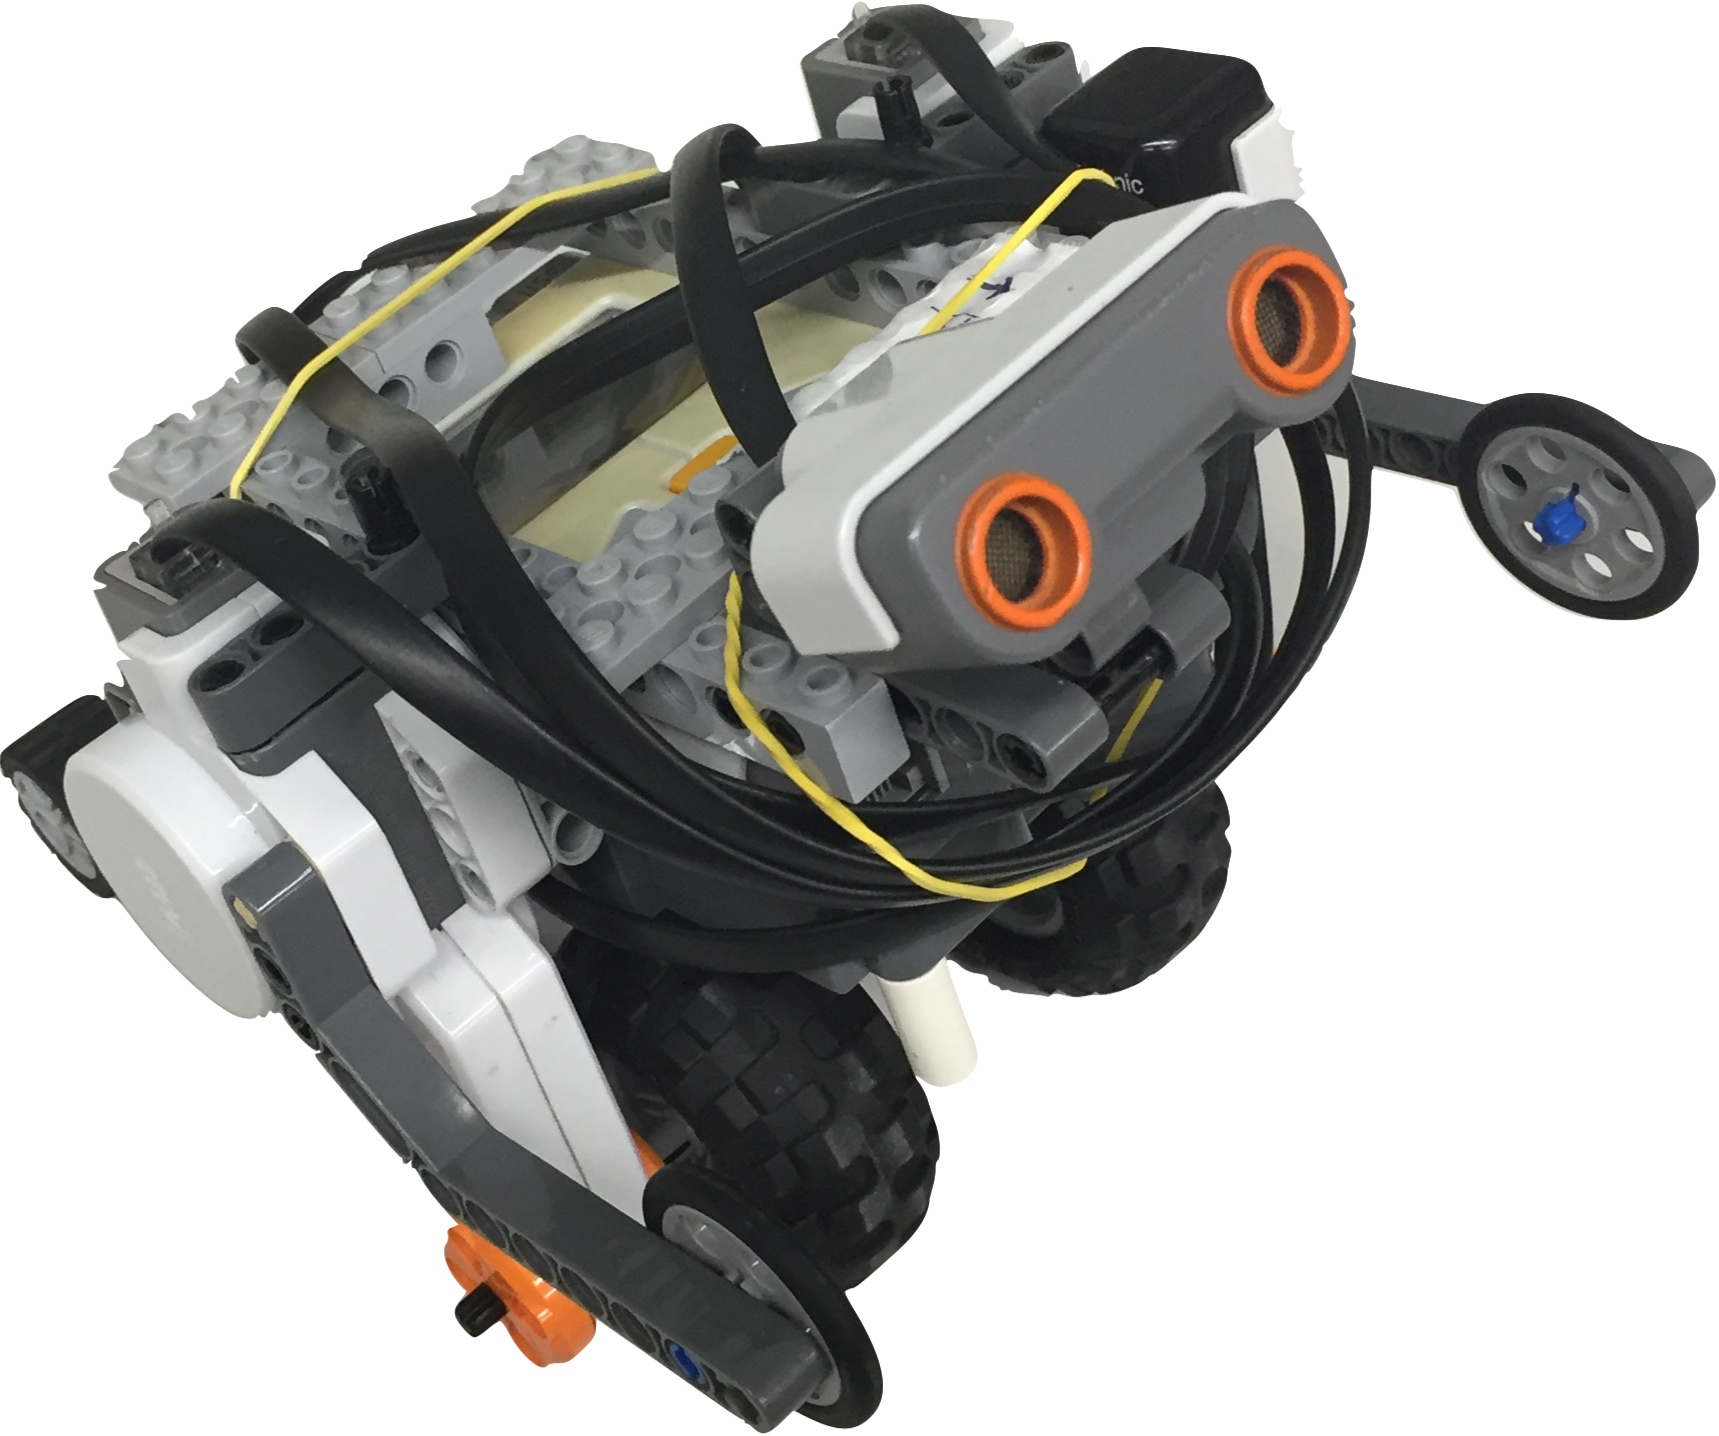
\includegraphics[width=0.38\textwidth]{NXT_3.jpg}
  \end{center}
  \caption{Aufbau Segway}
\end{wrapfigure}
%TODO besseres Foto
Der physische Aufbau unseres Roboters kam maßgeblich durch Ernüchterung über die verfügbaren Bauteile sowie falsches Priorisieren von bestimmten Eigenschaften zustande. 
Anfänglich überprüften wir verschiedene Konzepte nach denen der Aufbau sich richten sollte, beispielsweise den Brick so weit oben wie möglich zu platzieren um dessen Masse zum Vorteil beim Balancieren zu nutzen. Ähnlich dem Prinzip des Balancierens eines Besens mit einer Hand. Des weiteren vermuteten wir, dass die gesamte Struktur so stabil und verwindungssteif wie nur irgend möglich sein müsse. Dazu kamen selbstverständlich noch die Vorgaben der Kunden, dass der Brick nicht höher als 13cm sitzen darf sowie ausreichend Sturzbügel.

Nach nur wenigen Tests mit der LeJOS Segoway-Beispielklasse wurden schnell Komplikationen deutlich. Ein kopflastiger Roboter lässt sich zwar theoretisch einfacher balancieren, allerdings muss dafür mit ausreichender Geschwindigkeit auf Fallbewegungen reagiert werden, was mit den verfügbaren Motoren schlicht nicht möglich ist. Deren Schlupf sowie Ansprechverhalten ist dafür zu schlecht. Eben diese Nachteile waren es auch welche uns zwangen Räder mit lediglich 5,6 cm Durchmesser zu wählen, da dort das Spiel der Motoren durch den geringeren Umfang weniger ins Gewicht fiel. Wir nahmen den resultierenden Nachteil einer geringeren Höchstgeschwindigkeit in Kauf da der gewählte Umfang den besten Kompromiss bot. Des weiteren entschieden wir uns für eine standardmäßige Montage der Räder auf der Innenseite der Achsen. Dies ermöglicht ein deutlich schnelleres Drehen um die eigene Achse. Das Auslesen von korrekten und sinnvollen Daten aus dem, uns zur Verfügung stehenden, Gyrosensor erwies sich als sehr schwierig, weshalb wir wert darauf legten, dass dieser möglichst fest, direkt und schwingungsfrei befestigt wurde.
Der letztendliche Aufbau wurde so vor allem nach den Kriterien Einfachheit, Gewichtsreduzierung und Balancierfreudigkeit geschaffen.

\section{Projektorganisation}

Die Organisation des Projekts wurde hauptsächlich durch äußere Bedingungen bestimmt. Es wurde eine vereinfachte Form des Scrums für die Struktur vorgegeben. Als Scrum-Master wurde Gregor Kobsik bestimmt. Unser Team bestand aus fünf Mitglieder, wobei das Praktikum mit 6 ECTS Punkten angerechnet wird, was einem Arbeitsaufwand von 180h pro Mitglied entsprechen soll. In Anbetracht dessen, dass das Praktikum während des Semesters neben anderen Veranstaltungen nur ein Fünftel der regulären Arbeitszeit in Anspruch nehmen sollte, entschieden wir uns für eine mittlere Arbeitszeit von 8h pro Woche und Teammitglied. Das entspricht einem Aufwand von 120h im Verlauf des gesamten Praktikums bis zum Abschlussvortrag. Die geforderte und die tatsächlich zur Verfügung stehende Arbeitslast stehen schon am Anfang des Projekts im Widerspruch. Eine additive Arbeitszeiterfassung eines Teammitglieds sieht man in \Cref{fig:Arbeitszeiterfassung}.

Um die Anforderungen trotzdem zu erfüllen, entschieden wir uns dazu, Redundanz zu minimieren, Schnittstellen zwischen einzelnen Komponenten klar zu definieren und so eine parallele Entwicklung von Features, trotz ihrer gegenseitigen Abhängigkeit, zu ermöglichen. Infolgedessen spezialisierten sich die Mitglieder des Teams auf einzelne Aspekte ihrer Arbeit, wie GUI, Regler oder die Kommunikation. So konnten einzelne Personen zwei Wochen lang, trotz der üblichen wöchentlichen Fristen, für eine Abnahme arbeiten, indem sie sich schon frühzeitig mit den geforderten Anforderungen auseinandersetzten. Hierdurch konnte der Zeitaufwand auch sehr gut im Voraus approximiert werden und die benötigten Ressourcen bei Bedarf umverteilt werden. Das Konzept fand seinen Höhepunkt in der Implementierung der zusätzlichen Features, der Navigation und dem evolutionären Algorithmus für den Regler, die vollkommen autonom voneinander in der Entwicklung und Funktionalität sind. 

Des Weiteren muss man anmerken, dass alle Teammitglieder bei jedem Meeting anwesend waren. Dies erleichterte die Organisation und führte dazu, dass jeder sich an den Diskussionen und Grundsatzentscheidungen beteiligen konnte. Es wurden alle internen Deadlines eingehalten, wodurch die einzelnen Features problemlos ineinander eingebunden werden konnten.

\begin{figure}
	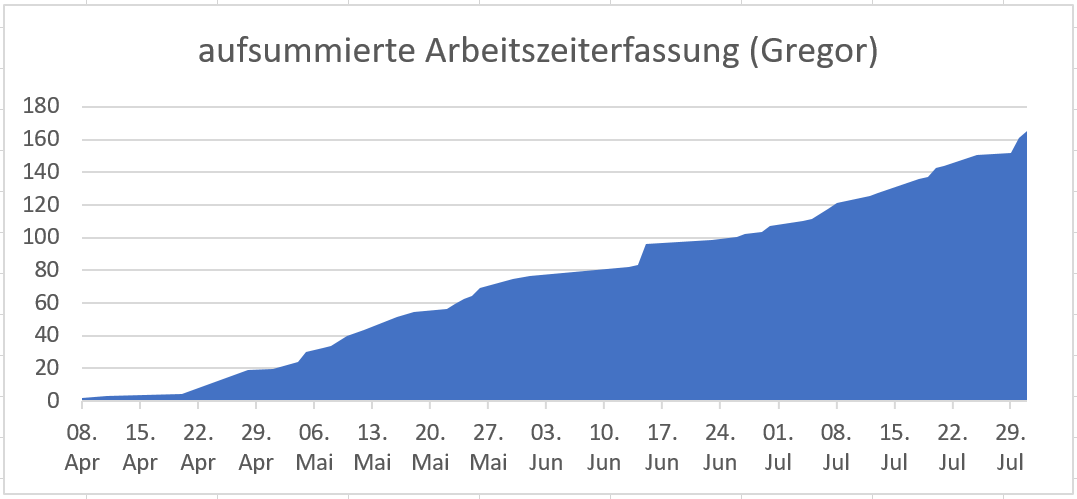
\includegraphics[width=\textwidth]{Arbeitszeiterfassung.PNG}
    \caption{Aufsummierte Arbeitszeiterfassung von Gregor Kobsik.}
    \label{fig:Arbeitszeiterfassung}
\end{figure}

\subsection{Zentrale Konzepte}

Den Mittelpunkt der Projektorganisation stellten die wöchentlichen Meetings dar. In diesen Meetings wurden nicht nur die vergangenen und zukünftigen Aufgaben besprochen, sondern auch Ideen ausgetauscht und Verbesserungen zur Implementierung kommuniziert. Der Erfolg der Meetings lässt sich auf eine feste Struktur zurückführen, die zunächst eine Agenda vor jedem Meeting voraussetzt. Ein weiterer Kernpunkt ist die Protokollführung. Jedes Treffen wurde abwechselnd von einem Teammitglied protokolliert. 
Das Protokoll bündelte unsere Entscheidungen in einem Dokument und wurde innerhalb von 24h in unserem internen Wiki veröffentlicht. Eine feste Struktur lässt sich auch innerhalb eines Meetings wiederfinden. Es wurde von dem Scrum-Master vorbereitet und geleitet, wobei es durch wiederkehrende Tagesordnungspunkte gegliedert worden ist. Jedes Treffen fing mit einer Eröffnung an, gefolgt von der Verlesung des letzten Protokolls, den vergangenen Aufgaben, der vergangenen Präsentation, sowie der Aufteilung der zukünftigen Aufgaben und der zukünftigen Präsentation. Es folgte der Tagesordnungspunkt Sonstiges und das Meeting wurde durch die Verlesung des aktuellen Protokolls beendet.

Ein weiteres Kernkonzept der Organisation stellt Pair Programming dar. Es zeichnet sich durch Partnerarbeit aus; hierbei programmiert eine Person, während die andere daneben sitzt und den Programmierer bei der Arbeit beobachtet. Auch wenn sie in erster Linie nicht aktiv programmiert, so dient sie vor allem der Qualitätssicherung. Sie muss sowohl den Code verstehen können, als auch mögliche Fehler direkt entdecken. Dies verkürzt im Anschluss die Fehlersuche und bietet ein simultanes Code Review. Darüber hinaus werden die Kernkonzepte gemeinsam besprochen und es fließen gemeinsame Ideen in die Implementierung. Studien belegen eine tatsächliche Verbesserung der Codequalität, sowie weitere Lerneffekte für beide Beteiligten, da sie ihre Erfahrungen direkt bei der Arbeit austauschen können. %TODO: include ref für eine Studie

Die treibende Kraft für die Entwicklung des NXT-Roboters stellten die Abnahmen dar. Jede Abnahme hatte einen fest definierten Funktionsumfang, den wir erfüllen mussten. Da die zu erfüllenden Aufgaben ausreichend genau spezifiziert worden sind, konnten wir testorientiert entwickeln. Zu jeder Abnahme haben wir eine Reihe an Tests definiert, die unser Roboter zunächst intern und danach extern in der Abnahme bestehen musste. Die Implementierung orientierte sich hierbei auf der Erfüllung der Funktionalität. Die folgende Behebung der potentieller Fehler orientierte sich hingegen an der Erfüllung der von uns definierten Tests.

\subsection{Weitere Konzepte}
\label{subsec:addConcepts}

Ein weiteres Konzept, das am Anfang sehr erfolgreich angewendet wurde, ist das Planing Poker. Hierbei schätzt jedes Teammitglied mittels spezieller Karten den Arbeitsaufwand in Stunden für ein Feature. In unserem Fall verwendeten wir die Karten mit 1, 2, 3, 5 und 8 Augenzahlen. Die Karten werden verdeckt gelegt und dann gleichzeitig umgedreht. Die Personen mit den niedrigsten und höchsten Zahl muss seine Entscheidung motivieren und so eine Diskussion anfangen. Dies ist ein iteratives Verfahren, das in unserem Fall schnell terminierte und gleichzeitig durch die Diskussion ein natürliches Brainstorming hervorbrachte. Das Verfahren fand keine Anwendung mehr, nachdem wir für eine Abnahme den vollständigen Zeitplan erstellten, da wir hierfür eine ausführliche Diskussion zu jedem Thema führen mussten. Hierdurch verlor das Projekt einiges an Dynamik, da wir uns einer statischen Durchführung des vorgegebenen Plans widmeten. \Cref{fig:Zeitplan} zeigt den initialen Zeitplan, wobei auf der y-Achse die Issues bzw. der organisatorische Aufwand eingetragen ist. Die x-Achse stellt den zeitlichen Verlauf und die Flächen die geschätzte Verteilung der Zeit auf die einzelnen Aufgaben, wobei die Diskretisierung auf 2,5h pro Flächeneinheit gewählt wurde.

\begin{figure}
	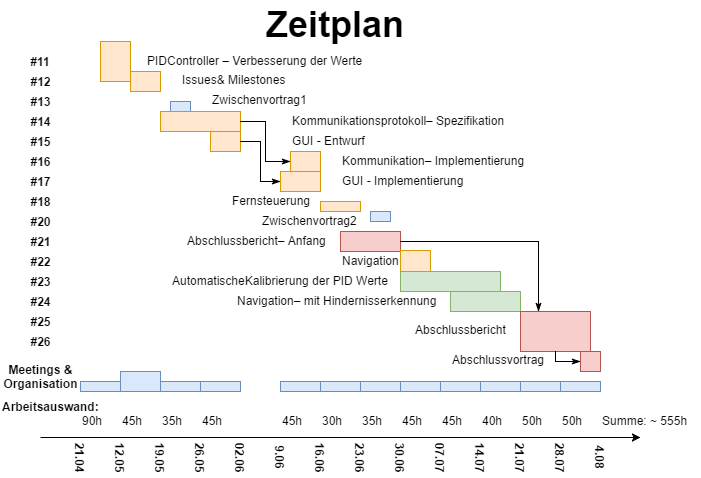
\includegraphics[width=0.9\textwidth]{Softwareprojekt-NXT-Zeitplan.png}
    \caption{Initialer Zeitplan für die Erfüllung der Aufgaben.}
    \label{fig:Zeitplan}
\end{figure}

Neben den vorherigen Konzepten gehört auch \texttt{GitLab} als Verwaltungs- und Organisationswerkzeug dazu. Durch \texttt{GitLab} konnten wir die benötigten Issues erstellen und uns so immer an einer aktuellen Übersicht über die zur Durchführung benötigten Schritte orientieren. Zusätzlich erlaubte es eine Nachverfolgung der aufgewendeten Zeit für die einzelnen Teilaufgaben. Das Wiki ermöglichte es uns, die Meetingprotokolle einfach zu veröffentlichen und allen Mitgliedern zur Verfügung zu stellen. Der größte Vorteil des \texttt{Git} ist allerdings die Versionskontrolle und Codeverwaltung. Hierdurch konnten wir durch die Branches an verschiedenen Features gleichzeitig und unabhängig voneinander arbeiten. Insbesondere erlaubte es uns, die Versionskontrolle auf Features auszulagern und erst später in den Hauptcode einzubinden, nachdem diese getestet wurden und ein Review passierten. Als Git-Workflow verwendeten wir Feature-Branches. Die Entwicklung eines Features fand also ausschließlich in einem dazu angelegten Branch statt, der \texttt{master}-Branch enthält nur Merge-Commits. Das Arbeitswerkzeug erlaubte zudem, auch überflüssige Elemente wie beispielsweise ein Dateiverwaltungssystem für den NXT zu implementieren, aber nie einzubinden, da im späteren Verlauf des Projekts keine sinnvolle Verwendung dafür gefunden wurde.

%TODO: irgendetwas fehlt, aber was?

\section{Regler}
\label{sec:Regler}
\begin{sloppypar}
Als Grundlage für den von uns entwickelten Regler diente die \texttt{Segoway}-Klasse von \ac{lejos}. Deren Regler besteht im wesentlichen aus einem PD- und einem PI-Regler mit den Einflussgrößen Neigungswinkel \texttt{gyroAngle}, Winkelgeschwindigkeit \texttt{gyroSpeed}, zurückgelegter Strecke  \texttt{motorPos}, Geschwindigkeit \texttt{motorSpeed} sowie der Zielgeschwindigkeit \texttt{motorControlDrive}.
%simpel und konkret. Passt.
Der \texttt{Segoway}-Regler weist einige Schwächen auf. Beispielsweise fängt der NXT beim Balancieren an zu \glqq wandern\grqq{}, also sich über Zeit immer weiter von seiner Startposition zu entfernen, ohne dazu angewiesen worden zu sein. 
%Lässt sich vllt besser schreiben.
%Besser so?
%ja
Durch eigene Test konnte dieses Verhalten darin begründet werden, dass \texttt{Segoway} die Winkelgeschwindigkeiten des Gyros aufaddiert um den Neigungswinkel des NXT zu berechnen. Wie in \cref{subsec:hardware} erläutert, ist dieser Winkel fehlerbehaftet und der Fehler wächst mit der Zeit. Um die Abweichung in der Neigung zu Kompensieren vergrößert der \texttt{Segoway}-Regler die Distanzabweichung in die entgegengesetzte Richtung und \glqq wandert\grqq{} folglich.

Als Konsequenz entwickeln wir unseren eigenen Regler von Grund auf, übernahmen aber sinnvolle Konzepte des \texttt{Segoway}-Reglers wie die Fall-Detection und den grundlegenden Aufbau des Reglers. Die Funktionalität ist in zwei Klassen aufgetrennt worden, nämlich \texttt{Sensordata}, welche sich um die Erhebung der Sensordaten kümmert, sowie \texttt{MotorController}, welche den eigentlichen Regler beinhaltet. \Cref{fig:pid} zeigt ein vollständiges Block-Diagramm unseres Reglers. Abgesehen von \texttt{distanceTarget} und \texttt{headingTarget}, welche Soll-Zustände für die Navigation darstellen, gibt es nur noch vier Einflussgrößen für den Regler.

\begin{figure}
  \tikzset{%
    saturation block/.style={draw, path picture={
        % Get the width and height of the path picture node
        \pgfpointdiff{\pgfpointanchor{path picture bounding box}{north east}}%
          {\pgfpointanchor{path picture bounding box}{south west}}
        \pgfgetlastxy\x\y
        % Scale the x and y vectors so that the range
        % -1 to 1 is slightly shorter than the size of the node
        \tikzset{x=\x*.4, y=\y*.4}
        %
        % Draw annotation
        \draw (-1,0) -- (1,0) (0,-1) -- (0,1); 
        \draw (-1,-.7) -- (-.7,-.7) -- (.7,.7) -- (1,.7);
      }
    }
  }
  \begin{tikzpicture}[auto, node distance=2cm,>=latex']
      \tikzstyle{every node}=[font=\small]
      \tikzstyle{block}=[draw, fill=white, rectangle, minimum height=3em, minimum width=3em]
      \tikzstyle{sum}=[draw, fill=white, circle, node distance=1cm]
      
      \coordinate(GSin) at (-2,-1) {};
      \coordinate[right of=GSin, node distance=2cm] (GSsplit) {};
      \draw (GSin) -- node{\texttt{gyroSpeed}} (GSsplit);

      \node[block] (GSi) at (2,-0) {$\displaystyle\sum_{k=0}^t g_s(k) \cdot 0.99^{t-k}$};
      \draw[->] (GSsplit) |-  node[above,pos=0.6]{$g_s(t)$}(GSi);
      \node[block,font=\tiny,align=center] (GSip) at (5.25,0) {\texttt{WEIGHT}\\\texttt{GYRO\_INTEGRAL}};
      \draw[->] (GSi) |- (GSip);
      \node[block,font=\tiny,align=center] (GSp) at (4.5,-2) {\texttt{WEIGHT}\\\texttt{GYRO\_SPEED}};
      \draw[->] (GSsplit) |- (GSp);

      \coordinate(MSin)  at (-2.5,-5) {};
      \coordinate[right of=MSin, node distance=2.5cm] (MSsplit) {};
      \draw (MSin) -- node{\texttt{motorDistance}} (MSsplit);

      \node[sum] (MSdiff) at (1,-4) {};
      \draw[->] (MSsplit) |- (MSdiff);
      \draw[->] ($(-0.8,0.75cm)+(MSdiff)$)node[left]{\texttt{distanceTarget}} -| node[pos=0.99] {$-$}(MSdiff);
      \node[saturation block, minimum width=1cm, minimum height=1cm](mspclamp) at (2.5,-4) {};
      \draw[->] (MSdiff) -- (mspclamp);
      \node[block,font=\tiny,align=center] (MSp) at (4.5,-4) {\texttt{WEIGHT}\\\texttt{MOTOR\_DISTANCE}};
      \draw[->] (mspclamp) -- (MSp);
      \node[block] (MSd) at (2,-6) {$\frac{m_d(t) - m_d(t-4)}{4}$};
      \draw[->] (MSsplit) |- node[below,pos=0.7]{$m_d(t)$} (MSd);
      \node[block,font=\tiny,align=center] (MSdp) at (5.25,-6) {\texttt{WEIGHT}\\\texttt{MOTOR\_SPEED}};
      \draw[->] (MSd) |- (MSdp);

      \node[sum] (powerRaw) at (6.5,-3) {};
      \draw[->] (GSip) -| (powerRaw);
      \draw[->] (GSp) -| (powerRaw.north west);
      \draw[->] (MSp) -| (powerRaw.south west);
      \draw[->] (MSdp) -| (powerRaw);

      \node[sum] (hdiff) at (8,0) {};
      \draw[->] ($(0,1.5cm)+(hdiff)$)node[above]{\texttt{heading}} -- (hdiff);
      \draw[->] ($(2,0.25cm)+(hdiff)$)node[above]{\texttt{headingTarget}} |- node[pos=0.99,below] {$-$}(hdiff);
      \node[saturation block, minimum width=1cm, minimum height=1cm](hclamp) at (8,-1) {};
      \draw[->] (hdiff) -- (hclamp);
      \node[block] (Hp) at (10,-1) {$W_{m_d}$};
      \draw[->] (hclamp) -- (Hp);

      \coordinate (Hpsplit) at (10,-2) {};
      \draw (Hp) -- (Hpsplit);
      \node[sum] (powerLeft) at (9,-4) {};
      \draw[->] (Hpsplit) -| (powerLeft);
      \node[sum] (powerRight) at (11,-4) {};
      \draw[->] (Hpsplit) -| node[pos=0.99] {$-$} (powerRight);

      \draw[->] (powerRaw) -| node[above,pos=0.3]{\texttt{rawPower}} (8,-3) -- (powerLeft);
      \draw[->] (8,-3) -| (10,-3) -- (powerRight);

      \node[saturation block, minimum width=1cm, minimum height=1cm](plclamp) at (9,-5.5) {};
      \draw[->] (powerLeft) -- (plclamp);
      \draw[->] (plclamp) -- ($(0,-1.5cm)+(plclamp)$) node[below]{\texttt{powerLeft}};
      \node[saturation block, minimum width=1cm, minimum height=1cm](prclamp) at (11,-5.5) {};
      \draw[->] (powerRight) -- (prclamp);
      \draw[->] (prclamp) -- ($(0,-1.5cm)+(prclamp)$) node[below]{\texttt{powerRight}};
  \end{tikzpicture}
  \caption{Wirkungsplan des PID.}
  \label{fig:pid}
\end{figure}
%Diagramm ist super!
\texttt{gyroSpeed} ist die aktuelle Winkelgeschwindigkeit des Gyro-Sensors. Im Gegensatz zum \texttt{Segoway}-Regler keine eigene Rekalibrierung des Gyro-Sensors durch, da \texttt{GyroSensor.getAngularVelocity} bereits selbst alle fünf Sekunden eine Rekalibrierung vornimmt, um der Drift entgegenzuwirken.

\texttt{gyroIntegral} ist kein eigentlicher Winkel mehr, sondern ein gedämpftes Integral. Dies hat den entscheidenden Vorteil, dass die Drift des Winkels in der Dämpfung verschwindet. Der Null-Winkel stellt sich somit an der Neigung ein, in der sich der NXT die meiste Zeit befindet, was die aufrechte Position ist. Eine starke, plötzliche Auslenkung wird dadurch gut erkannt und kann korrigiert werden. Eine andere Methode, die versucht wurde, um mit der Drift umzugehen, war die Verwendung eines zeitlich beschränkten Integrals über die Winkelgeschwindigkeiten der letzten $n$ Ticks. Aufgrund des erhöhten Speicherverbrauches um die letzten $n$ Winkelgeschwindigkeiten vorzuhalten, erwies sich diese Methode weniger effektiv. 

\texttt{motorSpeed} ist wie beim \texttt{Segoway}-Regler der Durchschnitt der Differenz in der \texttt{motorDistance} über die letzten vier Ticks.

\texttt{motorDistance} wird einerseits verwendet, um den NXT an einer Stelle zu halten und Positionsänderung durch Ausgleichsbewegungen auszugleichen, andererseits wird hierüber die Bewegung gesteuert. Der Regler versucht die Differenz zwischen \texttt{motorDistance} und \texttt{distanceTarget} zu minimieren. Durch das Setzen von \texttt{distanceTarget} kann somit eine Bewegung erzwungen werden. Die Differenz wird auf das Intervall $[-\texttt{MAX\_DISTANCE\_INFLUENCE}, \texttt{MAX\_DISTANCE\_INFLUENCE}]$ beschränkt, um zu verhindern, dass ein großer Wert für \texttt{distanceTarget} den Regler zu einer entsprechenden Reaktion veranlasst, welche ein Balancieren unmöglichen  machen würde. Als ein guter Wert für \texttt{MAX\_DISTANCE\_INFLUENCE} haben sich \SI{15}{\centi\meter} herausgestellt.

Um wechselnde Batteriespannungen zu kompensieren, wurde ein Skalierungsfaktor von $\SI{7.5}{\volt}/\texttt{Battery.getVoltage()}$ eingeführt. Der Wert von \SI{7.5}{\volt} wurde gewählt, da unter \SI{7}{\volt} der NXT in vorherigen Tests träge reagierte und nicht in der Lage war, über einen längeren Zeitraum aufrecht zu stehen. 

Für die Lenkung existiert analog zu \texttt{distanceTarget} ein \texttt{headingTarget}. Der Regler minimiert ebenso die Differenz von \texttt{heading} zum \texttt{headingTarget} und durch Setzen von \texttt{headingTarget} wird eine entsprechende Drehung ausgelöst.
\end{sloppypar}
%Sprache ist simpel und konkret. passt. Inhaltlich keine Fehler.
\subsection{Automatische Kalibrierung der Gewichte}
\label{subsec:autoPID}

Das sich unser Regler von dem \texttt{Segoway}-Regler unterscheidet und andere Eingangsgrößen verwendet, mussten wir neue Gewichte für die jeweiligen Werte finden. Eine Simulation kam nicht infrage, da keiner von uns besondere Erfahrung mit Regelungstechnik hatte und das System viele Unbekannte wie den Schlupf der Reifen, die Leistung der Motoren in Abhängigkeit der Akkuspannung oder die Genauigkeit des Gyro-Sensors aufweist. Das händische Einstellen der Regler-Gewichte stellte sich als mühsam und umständlich heraus. Daher wählten wir die automatische Kalibrierung der Gewichte als eines unserer Extras.
%die letzten drei Sätze lassen sich vllt etwas eleganter ausdrücken
\begin{wrapfigure}{l}{0.5\textwidth}
  \begin{tabular}{|c|l|}\hline
    \textbf{Zeit} & \textbf{Aktion}\\\hline
    -00:05 - 00:00 & stillstehen (standard PID)\\
    00:00 - 00:01 & stillstehen (neue Werte)\\
    00:01 - 00:06 & fahre \SI{20}{\centi\meter} nach vorne\\
    00:06 - 00:08 & drehe um \SI{180}{\degree}\\
    00:08 - 00:13 & fahre \SI{20}{\centi\meter} nach vorne\\
    00:13 - 00:15 & drehe um \SI{-180}{\degree}\\
    00:15 - 00:18 & fahre \SI{10}{\centi\meter} nach vorne\\
    00:18 - 00:20 & drehe um \SI{-180}{\degree}\\
    00:20 - 00:23 & fahre \SI{10}{\centi\meter} nach vorne\\
    00:23 - 00:25 & drehe um \SI{180}{\degree}\\\hline
  \end{tabular}
  \caption{Ablaufplan der automatisierten Tests.}
  \label{fig:evo_test}
\end{wrapfigure}
% TODO: bessere beschreibung für beschreibung

Ein großes Problem der händischen Kalibrierung war, dass es kein Unterscheidungsmerkmal gab, woran sich entscheiden ließe, welches von zwei Gewichten besser ist. Darum entwarfen wir einen festen Testablauf von \SI{25}{\second} Dauer, welcher in \Cref{fig:evo_test} zu sehen ist. Dieser Testablauf kann automatisch ausgeführt werden. Während des Tests sammelt der NXT Daten und übermittelt nach Ende des Tests an den PC. Ein Test endet entweder nach \SI{25}{\second} oder sobald der NXT umgefallen ist. Die gesammelten Daten sind die durchschnittliche Batteriespannung, durchschnittliche Abweichung von \texttt{distanceTarget} und \texttt{headingTarget}, sowie die aufrecht gestandenen Zeit. Diese Daten zusammen mit den vier Gewichten für den Testlauf bilden ein 8-Tupel, welches in einer CSV-Datei für die spätere Auswertung gespeichert wird. Zur Auswahl der durchzuführenden Testläufe wurden zwei Algorithmen implementiert.

\subsubsection{Binäre Suche}

Bei der Optimierung über binäre Suche wird jedes Gewicht separat maximiert. Da der Einfluss der einzelnen Gewichte nicht unabhängig ist, ist es notwendig alle Gewichte wiederholt zu optimieren, bis nur noch wenig Änderung eintritt.

Um ein Gewicht zu optimieren, wird der bisherige Wert $x_{old}$, sowie ein $\varepsilon_i$ betrachtet. 
Es werden drei Testläufe $x_i$, $x_i - \varepsilon$ und $x_i + \varepsilon$ durchgeführt. Der Wert mit dem besten Testergebnis wird übernommen und $\varepsilon_i$ halbiert, woraus sich die Iterationsvorschift
\begin{equation*}\begin{split}
x_0 &= x_{old}\\
\varepsilon_0 &= x_{old}\\
x_{i+1} &= \argmax_{x \in \{x_i,\,x_i - \varepsilon_i,\,x_i + \varepsilon_i\}} fitness(x)\\
\varepsilon_{i+1} &=  \frac{\varepsilon_i }{2}
\end{split}\end{equation*}
ergibt. Die Konvergenz dieses Verfahrens ist quadratisch, wodurch sich eine geringe Anzahl an Testläufen ergibt.

In der Praxis stellte sich heraus, dass die Testergebnisse sehr stark streuen und einzeln für sich nicht gut reproduzierbar sind. Dadurch läuft die binäre Gefahr, sich sehr schnell einmal für die falsche Seite zu entscheiden und anschließend das Maximum nicht mehr finden zu können.

\subsubsection{Evolutionärer Algorithmus}

Im folgenden wird ein Set von PID-Gewichten als Individuum bezeichnet. Eine Population setzt sich aus einer Menge von Individuen zusammen.

Der Ablauf des evolutionären Algorithmus ist folgender: Zu Beginn wird eine Population erzeugt, welche sich zu \SI{20}{\percent} aus den besten Individuen aus der Datenbank und zu \SI{80}{\percent} aus zufälligen Mutationen der bereits in der Population enthaltenen Individuen zusammen setzt. Anschließend wird jedes Individuum getestet.

Für die nächste Generation werden die besten \SI{20}{\percent} der Population beibehalten, \SI{40}{\percent} werden durch Kreuzung der verbliebenen Individuen wieder aufgefüllt. Die restlichen \SI{40}{\percent} stammen aus zufälligen Mutationen. Der Evolutionsschritt wird für einige Generationen wiederholt.

Der evolutionärer Algorithmus zeigte sich im Gegensatz zur binären Suche weniger anfällig für die hohe Streuung der Testergebnisse und lieferte wesentlich diversere Testläufe. Dadurch konnte die Experimentalzeit effektiver genutzt werden und mehr verwertbare Daten entstanden.
%ich weiß nicht ob das Wort "diversere" existiert :D
% Tut es^^ https://de.wiktionary.org/wiki/divers
%ok ^^
\subsubsection{Auswertung}
Insgesamt wurden 811 Tests durchgeführt. Von diesen wurden 17 verworfen, deren durchschnittliche Akkuspannung unter \SI{6.6}{\volt} lag. Unterhalb dieser Spannung war der NXT, trotz Normalisierung der Spannung im Regler auf \SI{7.5}{\volt}, in keinem Testlauf in der Lage, aufrecht zu bleiben.
Diese Daten stammen zur Hälfte aus der ersten Testserie mit der binären Suche und zur anderen Hälfte aus der zweiten Serie mit dem evolutionärer Algorithmus. Die Daten können gemeinsam ausgewertet werden, da beide Verfahren nur eine Auswahl der Testläufe treffen, aber auf deren Ergebnis keinen Einfluss haben.

Bei der Auswertung wurde einheitlich \cref{eq:fitness} als Fitness-Funktion verwendet. Diese legt ein hohes Gewicht auf ruhiges Balancieren, wobei Umfallen in jedem Fall schlechter ist. Durch den linearen Einfluss der Zeit beim Umfallen kann auch bei schlechten Werten noch ein Aussage über deren relative Güte getroffen werden. 

\begin{equation}\label{eq:fitness}
fitness(t, \bar{U},\bar{\Delta}_{distance},\bar{\Delta}_{heading}) =
\begin{cases}
	t &: t < 25\\
    25 + \frac{75}{1 + \bar{\Delta}_{distance} + \bar{\Delta}_{heading}} &: \text{sonst}
\end{cases}
\end{equation}

Das Ergebnis der Auswertung, aufgeteilt nach jedem Gewicht ist in \cref{fig:evo_result} zu sehen. Die Fitness-Werte wurden jeweils nach Gewicht gruppiert und der Durchschnitt je Gruppe betrachtet. Per polynomischer Regression wurde für jedes Gewicht ein Optimum bestimmt. Für \texttt{WEIGHT\_GYRO\_INTEGRAL} ist diese Regression wenig sinnvoll, da während der Tests die linke Flanke des Optimums nicht gefunden wurde. Es lässt sich trotzdem ein obere Grenze von \SI{-20} für \texttt{WEIGHT\_GYRO\_INTEGRAL} in den Daten erkennen.

Die als Ergebnis der Gewichtsoptimierung gefundenen sind in \cref{tab:evo_result_final} dargestellt.

\begin{figure}
  \centering
  \subfloat[\texttt{WEIGHT\_GYRO\_SPEED}: Maximum der polynomischen Regression bei 3,11437.]{
    \begin{tikzpicture}
      \begin{axis}[ymin=0,ymax=32.5]
        \addplot table [x index = {0}, y index = {1}, col sep=semicolon]{gyroSpeed.csv};
        \addplot[domain = -5.5:0,dotted,restrict y to domain=-1:33.5]{0.8514773198*x^4 + 10.2699698304*x^3 + 36.8188626525*x^2 + 33.3835285545*x + 0.7255280055};
        \draw [dashed,red] ++(axis cs:-3.11437,0) -- ++(axis direction cs:0,23.7509);
      \end{axis}
    \end{tikzpicture}
  }
  \subfloat[\texttt{WEIGHT\_GYRO\_INTEGRAL}: Regression nicht sinnvoll.]{
    \begin{tikzpicture}
      \begin{axis}[ymin=0,ymax=32.5]
        \addplot table [x index = {0}, y index = {1}, col sep=semicolon]{gyroIntegral.csv};
      \end{axis}
    \end{tikzpicture}
  }\hfill
  \subfloat[\texttt{WEIGHT\_MOTOR\_DISTANCE}: Maximum der polynomischen Regression bei 0,105979.]{
    \begin{tikzpicture}
      \begin{axis}[ymin=0,ymax=32.5]
        \addplot table [x index = {0}, y index = {1}, col sep=semicolon]{motorDistance.csv};
        \addplot[domain = 0:0.35,dotted,restrict y to domain=-1:33.5]{13449.3656328045*x^4 - 8565.8155800581*x^3 + 1288.6696835792*x^2 - 48.5576593650*x + 25.2903318174};
        \draw [dashed,red] ++(axis cs:0.105979,0) -- ++(axis cs:0,26.1186);
      \end{axis}
    \end{tikzpicture}
  }
  \subfloat[\texttt{WEIGHT\_MOTOR\_SPEED}: Maximum der polynomischen Regression bei 0,238327.]{
    \begin{tikzpicture}
      \begin{axis}[ymin=0,ymax=32.5]
        \addplot table [x index = {0}, y index = {1}, col sep=semicolon]{motorSpeed.csv};
        \addplot[domain = 0:0.45,dotted,restrict y to domain=-1:33.5]{12686.6220495332*x^4 - 12416.0563095503*x^3 + 3328.1550522999*x^2 - 
 157.6416184087*x + 0.0725807325};
        \draw [dashed,red] ++(axis cs:0.238327,0) -- ++(axis cs:0,24.3954);
      \end{axis}
    \end{tikzpicture}
  }\hfill
  \caption{Fitness pro Gewicht.}
  \label{fig:evo_result}
\end{figure}

\begin{table}
  \begin{center}\begin{tabular}{|l|c|c|}\hline 
  \textbf{Gewicht}&\textbf{Alt}&\textbf{Neu}\\\hline
  \texttt{WEIGHT\_GYRO\_SPEED}&-2.8&-3.11437\\
  \texttt{WEIGHT\_GYRO\_INTEGRAL}&-13&-20\\
  \texttt{WEIGHT\_MOTOR\_DISTANCE}&0,15&0.105979\\
  \texttt{WEIGHT\_MOTOR\_SPEED}&0,225&0.238327\\\hline
  \end{tabular}\end{center}
  \caption{Optimale Gewichte nach der Auswertung.}
  \label{tab:evo_result_final}
\end{table}
%liest sich gut. Zwei drei Typos aber kann man inhaltlich so lassen.

\section{Architektur}

Das Gesamtprojekt gliedert sich in zwei Teilprojekte, das PC-Projekt auf PC-Seite und das NXT-Projekt auf NXT-Seite. Diese Unterscheidung wurde bereits sehr früh getroffen, da sich die Hardware und insbesondere die zur Verfügung stehende Software auf beider Seiten sehr unterscheidet (vgl. \cref{subsec:hardware}). Die Brücke zwischen den beiden Projekten bildet die abstrakte Kommunikationsklasse, von der beide Implementierungen der Kommunikation erben. Die entsprechenden UML-Diagramme sind im Appendix unter den  \Cref{fig:Overview,fig:AbstractCom,fig:NXT,fig:CommNXT,fig:GuiPC,fig:ConnPC,fig:evo,fig:nav,fig:data,fig:Gamepad} zu finden.

\subsection{NXT}

Für das NXT-Projekt wurde das prozedurale Paradigma gewählt. Bis auf Ausnahmen sind alle Methoden und Variablen als \texttt{static} deklariert. Klassen dienen nur zur logischen Strukturierung des Quellcodes und werden nicht instanziiert. Dies erlaubt der \ac{jvm}, mehr Optimierungen vorzunehmen. In Java können Methoden, die nicht \texttt{final} oder \texttt{static} sind, von Unterklassen überschrieben werden (Laufzeit-Polymorphie). Aus diesem Grund kann die Bindung der Methoden nicht durch den Compiler erfolgen, sonder geschieht zur Laufzeit, was zeitgleich einen Overhead erzeugt. Aufgrund der limitierten Rechenkapazität des NXT und Echtzeitanforderung des Balancierens ist es wichtig, unnötigen Overhead zu vermeiden. Der Verzicht auf Objektorientierung auf NXT-Seite brachte wenig Probleme mit sich, da durch die \ac{lejos} \ac{jvm} insgesamt nur wenige nutzbare Bibliotheks-Klassen zur Verfügung stehen und Lambda-Ausdrücke generell nicht unterstützt werden. Zudem kann jede Klasse einem Hardwarebestandteil eindeutig zugeordnet werden. Es ist nicht sinnvoll mehrere Objekte einer Klasse besitzen zu können, da die Erfüllbarkeit der Funktionalität an äußere Gegebenheiten gebunden ist.

Da auf dem NXT mehrere Threads gleichzeitig laufen, die sich gegenseitig jedoch nicht blockieren dürfen (z.B.: Kommunikation und Balancieren) wurde darauf geachtet, dass alle Threads die gleiche Priorität erhalten, da sonst ein höher priorisierter Thread die anderen blockieren kann (vgl. \cref{subsec:hardware}).

\subsection{PC}

Für das PC-Projekt wurde auf die objektorientierte Programmierung gesetzt. Im Gegensatz zu dem NXT ist man auf der PC-Seite nicht durch die Hardware limitiert und kann einen Overhead zur Laufzeit in Kauf nehmen, wenn man hierdurch schneller und fehlerfreier das gewünschte Ergebnis erzielen kann. Schon die Implementierung der GUI benutzt Objekte, die wie z.B. Buttons mehrfach vorzufinden sind (vgl. \Cref{sec:Gui}). Auch die Verwendung von Interfaces ermöglichte uns eine intuitive Anbindung der Klassen an das vorhandene Eventsystem. Für eine gleichzeitige Ausführung verschiedener Aufgaben, wie der Kommunikation, der GUI oder der Navigation, wurden jeweils eigene Threads erstellt, die unabhängig voneinander arbeiten. Hierbei wurde darauf geachtet, alle Aufgaben, die rechenintensiv sind und nicht vom NXT übernommen werden müssen, auf den PC auszulagern. So wird die Navigation auf dem Rechner berechnet und lediglich ein Befehl für die Bewegung an den NXT übermittelt (vgl. \cref{sec:navigation}). Das PC-Projekt dient als ein logischer Master, der den NXT steuert. 
%TODO: "Schon die Implementierung der GUI benutzt Objekte, die wie z.B. Buttons mehrfach vorzufinden sind." Wie viel trägt der Satz zum Inhalt und Verständnis bei?
%TODO: sich über falsche implementierung von available() beschweren.

\section{GUI}
\label{sec:Gui}
Erste Konzepte für eine grafische Benutzeroberfläche wurden bereits frühzeitig im Verlauf dieses Projekt besprochen. Das Aufstellen des Lasten- sowie Pflichtenhefts war dabei von entscheidender Bedeutung, da hier der Umfang der notwendigen Funktionen deutlich wurde. Die drei wesentlichen Bereiche Überwachungsgrößen, Kommunikation und Funktionen wurden früh definiert sowie erste Lösungsansätze erarbeitet.\\
% Die Wahl der Namen ist nicht intuitiv zur Funktionalität. Überwachungsgrößen oben, Funktionalitäten sind abhängig vom Kontext im Tab View links gegeben, weitere Ausgaben, vor allem Kommunikationsnachrichten rechts im Textfeld. Zuerst die grobe Unterteilung in 3 Funktonsbereiche schildern, dann Details
\begin{figure}[!h]
	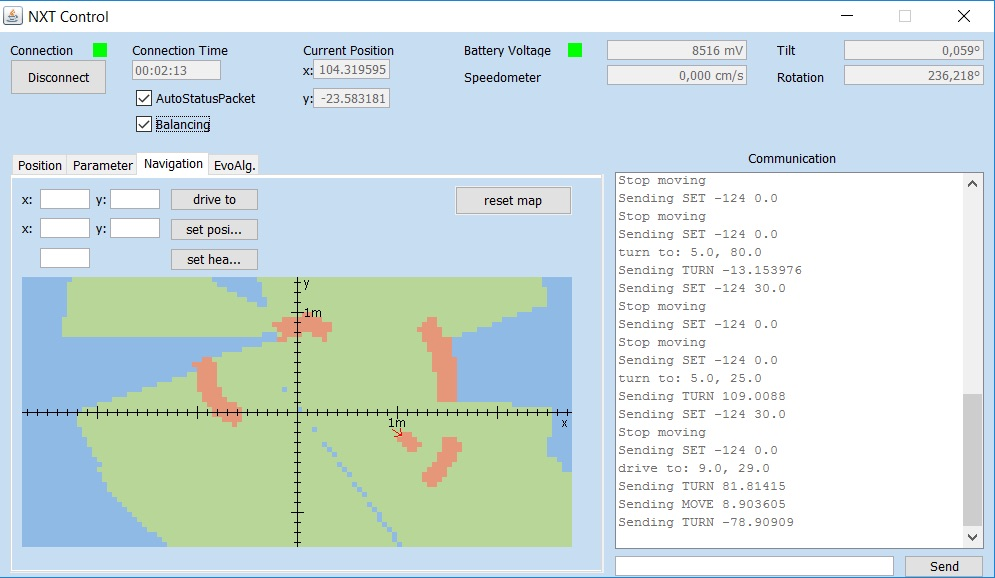
\includegraphics[width=\textwidth]{GUI_connected.jpg}
    \caption{GUI NXT Control}
    \label{fig:NXTControl}
\end{figure}
%zum besseren Verständnis Tab view oben auch mit in die Grafik inkludieren.
Die Namen sind trivial gewählt: \dq Überwachungsgrößen\dq(oben im Bild) zeigt Informationen, beispielsweise Batteriespannung, Neigung, Ausrichtung, Geschwindigkeit, Verbindungsdauer u.Ä., sowie alle nötigen Bedienelemente zum Verbindungsaufbau. \dq Kommunikation\dq(rechts) beschreibt schlichtweg eine Konsole mit Ein- und Ausgabefeldern die zum einen eine Bestätigung für getätigte Befehle und empfangene Daten ist, sowie die Möglichkeit bietet in Textform alle Bedienelemente der GUI manuell einzugeben. \dq Funktionen\dq(links) ist ein Reiterfeld das vor allem durch seine Modularität einen großen Umfang bietet wie etwa die Parametrierung(u.a. der PID-Werte) aber auch alle nötigen Felder und Bedienelemente zur Navigation und zum Fahren. Die Verwendung eines solchen Tab-Views erlaubt das Hinzufügen und Entfernen von Funktionen und Extras ohne das grundlegende Bedienkonzept der graphisches Benutzeroberfläche ändern zu müssen.\\
Die Oberfläche ist einheitlich in englischer Sprache geschrieben. Initial sind alle Buttons, außer dem \dq Connect\dq-Button, deaktiviert und werden erst bei erfolgreichem Verbindungsaufbau zu einem NXT freigegeben. Ab diesem Zeitpunkt beginnt die Uhr unter \dq Connection Time\dq\ zu laufen und da der NXT von sich aus Status Pakete beginnt zu verschicken werden auch die restlichen Informationsfelder befüllt. Die Beschriftung der Buttons in Kombination mit passenden Labels ermöglicht eine Verwendung der GUI ohne eine Einweisung des Nutzers. Es wurde an sinnvollen Stellen Checkboxen statt Buttons verwendet oder Dropdown-Menüs statt Freitextfeldern. Der Zugriff auf nicht erlaubte Felder wie beispielsweise dem Ausgabefeld der Konsole sind deaktiviert und der Nutzer wird bei unzulässigen Eingaben auf seinen Fehler hingewiesen.
\begin{wrapfigure}{r}{0.5\textwidth}
  \begin{center}
    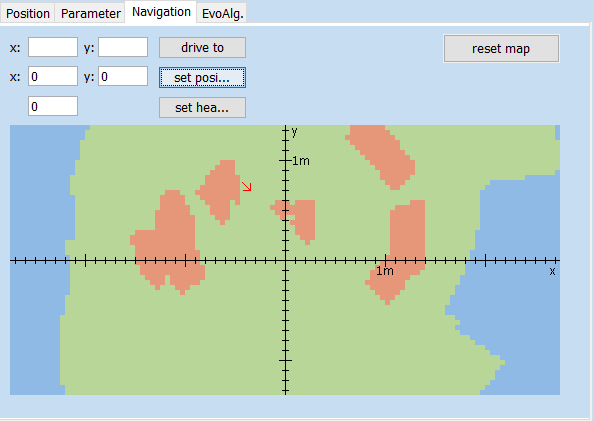
\includegraphics[width=0.48\textwidth]{navi_map.jpg}
  \end{center}
  \caption{Reiter Navigation}
\end{wrapfigure}
% Die Karte könnte ausgefüllt sein. TODO: Montags neues Bild
Dem Reiter \dq Navigation\dq kommt beim Arbeiten am NXT mit der GUI besondere Bedeutung zuteil. Die dargestellte Karte bietet eine Übersicht der Umgebung sowie die aktuelle Position. Der Ursprung des Koordinatensystems bildet der Punkt (0,0), welcher dem Startpunkt des NXT zum Beginn des Balancieren entspricht. Der NXT selbst wird durch einen roten Pfeil symbolisiert dessen Richtung der Ausrichtung des Roboters entspricht. Hierbei wird initial eine Ausrichtung in positiver Y-Achse angenommen. Des weiteren bietet der Reiter Bedienelemente zur Steuerung (z.B. drive to) oder auch zum manuellen Setzen der Position und der Ausrichtung. Interessant wird das Fenster vor allem in Kombination mit der Navigation mit Hinderniserkennung (vgl. \cref{subsec:navigationhinderniskarte}),
denn die erfassten Daten des Ultraschallsensors werden direkt in die Karte gespeist und farblich dargestellt. Auch hier wurde bei der Implementierung besonderes Augenmerk auf Intuitivität gelegt, so erlaubt die Karte eine interaktive Nutzung, indem der Benutzer über ein Mausklick die Position definieren kann, die der NXT anfahren soll.


\section{Kommunikation}
Um die Kommunikation zwischen NXT und PC zu realisieren, wurde gruppen"ubergreifend ein allgemeing"ultiges Kommunikationsprotokoll entworfen, das M"oglichkeiten zu gruppeninternen Erweiterungen offenl"asst. Da die endgültige Fassung dieses Protokolls zu großen Teilen auf unserem zuvor ausgearbeiteten Prototypen basiert, wird sie hier umfangreich vorgestellt. Das Protokoll spezifiziert dabei die Art der Daten"ubertragung und die allgemeine Codierung von Befehlen. Der Grundgedanke dieses Protokolls ist die Erm"oglichung einfacher Kommunikation zwischen PCs und NXTs, die von verschiedenen Gruppen stammen.
%TODO zweiten Satz (nachträglich hinzugefügt) drinlassen oder soll das weg?

\subsection{Allgemein}
Das allgemeine Kommunikationsprotokoll definiert die Datenübertragung als Stream-basiert über das \texttt{NXTComm}-Interface. Das Interface bietet mit dem Übertragungsmodus \texttt{PACKET} eine sichere Datenübertragung mit Header-Daten und umfangreiche Funktionalit"aten zum Verbindungsauf- und -abbau sowie zum Datenaustausch. Empfohlen wird hierbei die Verwendung von DataInput- und DataOutput-Streams für die Handler. Eine Implementierung soll eine "Ubertragungsrate von f"unf Commands pro Sekunde in beide Richtungen gew"ahrleisten k"onnen. Paketverluste sind nur bei hoher Auslastung auf der Seite des Slaves möglich und werden abh"angig von der Implementierung entweder ignoriert oder quittiert und dem PC angezeigt.

\subsubsection{Commands}
Wesentlicher Bestandteil des Kommunikationsprotokolls ist die allgemeing"ultige Codierung von Nachrichten. Eine Nachricht beginnt immer mit einem Command, gefolgt von eventuellem Payload, der beliebige L"ange haben kann, aber für jeden Command fest definiert ist. Der Handler eines Commands ist dafür verantwortlich, die richtige Anzahl an Bytes zu lesen, um eine korrekte Interpretation der Daten zu gewährleisten. Jeder Command wird in Form einer CommandID vom Typ byte codiert und einer Nachricht vorangestellt.

Die genaue Codierung der Commands, ihre Struktur und die Kommunikationsrichtung ist \cref{tab:cmdTable} im Anhang zu entnehmen.\\  

\noindent\textbf{Set}

Der erste allgemeing"ultige Command ist Set. Set wird vom PC and den NXT gesendet, um den Wert eines Parameters neu zu setzen und wird gefolgt von der Codierung eines zul"assigen Parameters sowie den zu setzenden Werten. \\ 

\noindent\textbf{Get}

Der Get-Command wird vom PC an den NXT gesendet, um den aktuellen Wert eines Parameters abzufragen, und wird ebenfalls von der Codierung eines zul"assigen Parameters gefolgt. \\

\noindent\textbf{GetReturn}

Der GetReturn-Command kennzeichnet die Antwort des NXT auf eine Get-Anfrage des PCs. Der GetReturn-Command wird vom NXT an den PC gesendet und wird von der Codierung des gefragten Parameters sowie den Werten gefolgt. \\

\noindent\textbf{Move}

Der Move-Command wird vom PC an den NXT gesendet und wird von einer Distanz in Zentimetern gefolgt, um die sich der NXT in gerader Richtung vorwärtsbewegen soll. \\

\noindent\textbf{Turn}

Der Turn-Command wird vom PC an den NXT gesendet und wird von einem Winkel in Grad gefolgt, um den sich der NXT nach links (mathematischer Drehsinn) drehen soll. \\

\noindent\textbf{MoveTo}

Der MoveTo-Command ist reserviert. Er war urspr"unglich dazu gedacht, den NXT dazu zu veranlassen, sich zu einer Koordinate zu bewegen. Das Navigieren zu einer Koordinate soll durch PC-interne Umrechnung über Move- und Turn-Commands realisiert werden. Als Konsequenz ist das Senden dieses Commands zurzeit ein Fehler. \\

\noindent\textbf{Balancing}

Dieser Command wird von einem Boolean gefolgt, der den NXT anweist, das Balancieren zu starten oder zu stoppen. True wird hierbei als Anweisung zum Starten interpretiert. \\

\noindent\textbf{LogInfo}

Der Command wird vom NXT zum PC gesendet, um kurze Nachrichten "ubermitteln zu k"onnen, die nicht über andere Commands realisierbar sind wie beispielsweise Debug-Nachrichten. Der String, der diesem Command folgt, wird in UTF-8 kodiert. \\

\noindent\textbf{ErrorCode}

Dieser Command überträgt spezifizierte Errors des NXT an den PC. \\

\noindent\textbf{Disconnect}

Dieser Command wird vom PC an den NXT gesendet, um einen sicheren Verbindungsabbau zu initialisieren. Der Verbindungsabbau ist in diesem Fall eindeutig erw"unscht. \\

\noindent\textbf{ProtocolVersion}

Dieser Command wird initial vom NXT zum PC gesendet und von einem byte gefolgt, welches die Protokollversion des NXT kodiert. Die Protokollversionen sind dabei intuitiv mit den Gruppennummern kodiert. Das allgemeine Kommunikationsprotokoll wird mit 0 kodiert. Der PC entscheidet nach Empfang dieses Commands, ob er nur die allgemeinen oder zus"atzlich die gruppenintern spezifizierten Commands und Parameter verwendet. Da gruppenfremde NXTs die internen Spezifikationen nicht kennen, f"uhrt ein Senden nicht-allgemeiner Commands und Parameter zu Fehlern in der Verarbeitung und ist daher illegal. \\

\noindent Die CommandIDs im Bereich von 128-255 sind für gruppeninterne Definitionen offen. Dies ermöglicht eine problemlose Erweiterung der allgemeingültigen Commands bei Bedarf, ohne Kollisionen mit internen Definitionen zu riskieren. Interne Erweiterungen der Commands können bei speziellen Extras notwendig sein, da in diesem Fall eine Erweiterung der allgemeingültigen Commands nicht sinnvoll ist.

\subsubsection{Error-Codes}
Ein ErrorCode-Command wird immer von einem codierten Error gefolgt. Allgemeing"ultige Error-Codes existieren zwei. Auch bei den Error-Codes ist der Bereich von 128-255 für gruppeninterne Erweiterungen offengelassen. \\

\noindent\textbf{NXTFallen}

Der NXT sendet diesen Error, wenn das Balancieren aufgeh"ort hat, ohne dass ein entsprechender Command gesendet wurde. \\

\noindent\textbf{PacketLoss}

Dieser Error kann vom NXT gesendet werden, wenn ein Paketverlust erkannt wurde und quittiert werden soll.

\subsubsection{Parameter}
Um grundlegende Kommunikation mit gruppenfremden NXTs zu ermöglichen, muss eine Schnittmenge an Parametern allgemeing"ultig kodiert werden. Dadurch k"onnen wesentliche Informationen des NXT wie Batteriespannung und Geschwindigkeit versionsunabh"angig abgefragt werden. Spezifischere Parameter, die beispielsweise bei der Gewichtung der Werte des Reglers eine Rolle spielen, werden hingegen gruppenintern im Bereich von 128-255 kodiert. Die genaue Kodierung der Parameter sowie Typ und Einheit ihrer Werte ist \cref{tab:paramTable} im Anhang zu entnehmen.\\

\textbf{BatteryVoltage/GyroAngle/TachoLeft/TachoRight}

Diese Parameter kennzeichnen die aktuellen Messgrößen der verwendeten Hardware. Da diese Hardware von jeder Gruppe verwendet wird, k"onnen die Parameter allgemeing"ultig definiert werden.\\

\noindent\textbf{Heading}

Dieser Parameter bezeichnet die aktuelle Ausrichtung des NXT in Grad. Seine Startposition ist hierbei als 0 definiert und die Ausrichtung im mathematischen Drehsinn nach links berechnet. \\

\noindent\textbf{Position}

Dieser Parameter kennzeichnet die aktuelle vom NXT berechnete Position als Koordinaten. Als Ursprung wird hierbei initial die Startposition festgelegt. \\

\noindent\textbf{MovementSpeed}

Die aktuelle, aus der Geschwindigkeit aller Motoren gemittelte Geschwindigkeit des NXT. \\

\noindent\textbf{StatusPacket}

Eine B"undelung mehrerer, h"aufig abgefragter Parameter, die Heading, Position und MovementSpeed beinhaltet. \\

\noindent\textbf{AutoStatusPacket}

Dieser Parameter erm"oglicht die Aktivierung und Deaktivierung automatischen Sendens von StatusPackets auf Seiten des NXT. \\

\noindent\textbf{PID-Gewichte}

Da die Anzahl und Art der PID-Gewichte stark implementierungsabh"angig ist, wurde f"ur diese nur ein Intervall bereitgestellt, ohne die Gewichte konkret zu benennen.

\subsection{Gruppeninterne Erweiterung}
Die gruppeninternen Erweiterungen der Commands beschr"anken sich auf das Definieren der CommandID 0 als invalide. Auch die Error-Codes wurden nicht erweitert.

\subsubsection{Parameter}
\textbf{GyroSpeed/GyroIntegral/MotorDistance/MotorSpeed}

Diese Parameter kennzeichnen die Gewichtung der PID-Werte. Zur konkreten Verwendung und dem Einfluss der PID-Werte siehe Kapitel Regler. \\

\noindent\textbf{WeightAll}

Dieser Parameter b"undelt, "ahnlich wie das StatusPacket, alle PID-Werte, um mit weniger Commands mehr Daten "ubertragen zu k"onnen. \\

\noindent\textbf{ConstantRotation/ConstantSpeed}

Diese Parameter erm"oglichen das Setzen und Abfragen einer konstanten Drehgeschwindigkeit oder Bewegungsgeschwindigkeit des NXT. Diese Option wird in der PC-internen Navigation nach Koordinaten genutzt, kann aber auch manuell verwendet werden. \\

\noindent\textbf{WheelDiameter/Track}

Diese Parameter erm"oglichen das Anpassen der NXT-Software an Hardwaremodifikationen. \\

\noindent\textbf{UltraSensor}

Dieser Parameter kennzeichnet Daten, die vom Ultraschallsensor ermittelt und "ubertragen werden. \\

\noindent\textbf{CollectTestData/Measurements}

Diese Parameter werden bei der automatischen Kalibrierung des PID-Reglers verwendet. CollectTestData startet dabei einen neuen Testdurchlauf und l"oscht die alten Daten, Measurements kennzeichnet gesammelte Daten, die vom NXT an den PC gesendet werden.


\section{Navigation}
\label{sec:navigation}
Die Navigation des NXT basiert auf der Steuerung. Für die Steuerung des NXT wurden vier Funktionen implementiert: \texttt{move}, \texttt{turn}, \texttt{constantSpeed}, \texttt{constantRotation}. Die Bewegung wurde über Manipulation des PID Reglers realisiert (vgl. \cref{sec:Regler}).

Der Befehl \texttt{move} bewegt den NXT um eine zuvor bekannte Distanz in einer geraden Linie. \texttt{turn} dreht den NXT um einen zuvor bekannten Winkel. \texttt{constantSpeed} beschleunigt den NXT auf eine bestimmte Geschwindigkeit, allerdings ohne mit der Bewegung aufzuhören. Diese Aktion wird über einen weiteren \texttt{constantSpeed} Befehl mit der Geschwindigkeit \texttt{0} realisiert. \texttt{constantRotation} funktioniert analog zu \texttt{constantSpeed}, verursacht aber eine Drehung des NXT.


%Für die Bewegungsfernsteuerung wurden zwei verschiedene Möglichkeiten implementiert. 
% Die stehen nicht zur Verfügung, die haben wir gemacht
%Dabei kann der NXT einerseits über die \glqq move\grqq\ und \glqq turn\grqq\ Standardbefehle bewegt werden, also kann sich der NXT um eine zuvor bekannte Distanz
% Besser: bestimmte Distanz. Zentimeter ist ein Implementierungsdetail und hier nicht relevant.
%in einer geraden Linie vor und zurück bewegen und um einen zuvor bekannten Winkel um die eigene Achse drehen. Dies ist durch die Manipulation des PID Reglers realisiert, zu sehen in \cref{sec:Regler}.
% Verweis auf Kapitel Regler, Erläuterung dort
%Da diese Art der Bewegungsfernsteuerung nur angewendet werden kann, wenn die jeweiligen Parameter bereits vor dem Senden des Befehls bekannt sind, verfügt der NXT über eine zweite Art der Bewegungsfernsteuerung.
% Das ist inhaltlich drei mal der gleiche Satz
%Diese Funktion ist über die zwei Parameter \glqq constantSpeed\grqq\ und \glqq constantRotation\grqq\ realisiert. Ist dort ein anderer Wert als null gespeichert, fährt oder dreht sich der NXT.
% Stimmt nicht: Feste Drehung und Bewegung immer noch möglich.
%Der konkrete Wert des Parameters entspricht dabei der Geschwindigkeit. Deswegen können diese Aktionen mit dem \glqq set\grqq\ Befehl ausgelöst werden.
% Statt Anführungsstrichen besser \texttt{...}
% Was heißt "Geschwindigkeit konstant aufgebaut"
%Mit diesen Varianten der Bewegungsfernsteuerung kann der NXT auf verschiedene Weisen navigiert werden.

%Besser: Für die Steuerung des NXT wurden vier Funktionen implementiert: move, turn, ... etc. und dann eine kurzer Erklärung der jeweiligen Funktion.

\subsection{Navigation mit der GUI}

In der GUI können die zuvor genannten Varianten der Bewegungsfernsteuerung ausgelöst werden. Für das Senden von \texttt{move} und \texttt{turn} Befehlen stehen im Tab \texttt{Position} zwei Buttons zur Verfügung, die die \texttt{move} und \texttt{turn} Befehle mit Parametern aus den nebenstehenden Textfeldern versenden. Ein dritter Knopf kann den NXT außerdem auf eine absolute Gradzahl ausrichten. Dies ist durch das Speichern und Aktualisieren von Daten, die der NXT an den PC sendet, realisiert. Wichtig für die Navigation sind dabei das Heading, also die aktuelle Ausrichtung, und die Position. Mit Hilfe der aktuellen Aurichtung wird die schnellste Drehung auf die gewünschte Gradzahl berechnet und durch einen \texttt{turn} Befehl ausgeführt. 

Ebenfalls im Tab \texttt{Position} befinden sich vier Knöpfe in Anordnung der Pfeiltasten einer Tastatur. Ist dieser Tab geöffnet reagiert die GUI auf die \texttt{W}, \texttt{A}, \texttt{S} und \texttt{D} der Tastatur und ordnet sie sinngemäß den Knöpfen der GUI zu.
% Fokus auf dem oberen Knopf nicht notwendig, es reicht den Tab offen zu haben
Diese Knöpfe steuern den NXT über die \texttt{constantSpeed} und \texttt{constantRotation} Funktionen.
% Muss das wirklich erklärt werden? :D
Die Geschwindigkeiten für Drehung und Fahren entsprechen dabei Konstanten, die so gewählt wurden, dass der NXT stabil bei seinen Bewegungen ist. Außerdem können diese Parameter über den Tab \texttt{Parameter} manuell gesetzt werden, wobei die Werte direkt den Geschwindigkeiten der Drehung und des Fahrens entsprechen. Daher wird nicht empfohlen von dieser Methode Gebrauch zu machen.
% Gut!
% MAX_DISTANCE_INFLUENCE und MAX_HEADING_INFLUENE können afaik PC-seitig nicht überschrieben werden, wodurch Limits existieren und keine Gefahr für die Stabilität ausgeht.

\subsection{Navigation mit dem Controller}
\label{subsec:Controller}

Um das manuelle Steuern des NXT für den Benutzer handlicher zu machen wurde zusätzlich eine Steuerung mit einem Gamepad implementiert. Diese wird durch die JInput Library möglich gemacht, die die Inputs eines Controllers abrufbar macht.
% Die verwendete library heißt JInput, Ivy dient nur zum einfacheren laden von libraries.
Dazu werden \texttt{constantSpeed} und \texttt{constatRotation} verwendet. Die Daten des linken Analogsticks sowie der beiden Trigger werden in einem regelmäßigen Takt abgerufen. Der rechte Trigger löst eine Bewegung nach vorne aus, während der linke Trigger eine Bewegung nach hinten auslöst. Die Daten des Analogsticks werden in eine Drehung nach links oder rechts umgesetzt, je nachdem in welche Richtung der Stick bewegt wird. Dabei wird sowohl bei den Triggern als auch bei dem Analogstick die Intensität der Aktion beachtet. Das bedeutet, dass ein schwächeres Drücken eines Triggers eine ebenso langsamere Bewegung an den NXT sendet. Um unnötige Befehle bei kleinen Intensitäten zu Filtern, werden Befehle nur bei einer Intensität von mindestens zehn Prozent gesendet. Die einzige Ausnahme bildet der Befehl zum stoppen einer Drehung oder einer Bewegung, der beim Unterschreiten dieser zehn Prozent einmalig gesendet wird. Erst bei einem erneuten Überschreiten werden neue Befehle bezüglich Bewegung gesendet. Es findet zudem eine Diskretisierung der abgetasteten werde in 20 Stufen statt, um dem analogen Rauschen entgegen zu wirken und so überflüssige Kommunikation zu vermeiden.
% Gut

\subsection{Navigation über die Karte mit Hinderniserkennung}
\label{subsec:navigationhinderniskarte}
Zunächst bestand die Navigation nach Koordinaten über eine Umrechnung, in der aus den aktuellen Daten und der gewünschten Position ein \texttt{turn} und ein \texttt{move} Befehl berechnet wurde, der diese Position direkt anfährt. Diese Funktion wurde durch eine komplexere Version ersetzt (vgl. \cref{subsec:pathfinding}), wird allerdings von dieser intern verwendet und ist daher nicht mehr direkt aufrufbar.
% Tut sich doch immer noch? Sonst: Navigation an Koordinaten nicht erklärt
Die GUI verfügt außerdem über eine Karte, in der die Position und die Ausrichtung des NXT angezeigt wird. Mit einem Klick auf die Karte wird ein Befehl zum Anfahren der entsprechenden Koordinate gesendet.
% Der Listener ist für die Funktionalität nicht relevant, es reicht das ein Klick in eine Bewegung umgesetzt wird
Der im NXT verbaute Ultraschallsensor sendet außerdem regelmäßig seine Daten an den PC, der aus diesen Daten die Positionen von Hindernissen ausließt und in einer internen Datenstruktur speichert. Das interne Setzen eines Hindernisses erfolgt über eine Lernrate. So ist eine dynamische Umgebung erfassbar und fehlerhafte \texttt{frei} Signale (vgl. \cref{subsec:hardware}) lassen den NXT nicht direkt in ein Hindernis fahren.
%Evtl. auf Kapitel Hardware verwiesen, da wird die Sensor-Problematik auch erklärt.
Zum Speichern wird die Karte in Quadrate mit \SI{5}{\centi\meter} Kantenlänge unterteilt, da die Ungenauigkeiten der Hardware keine genauere Diskretisierung nötig machen. Der Inhalt dieser Karte wird in regelmäßigem Abstand komplett auf die Karte der GUI gezeichnet, wobei zwischen bekannten und unbekannten Feldern unterschieden wird. Über der Karte befinden sich Knöpfe zum setzen von Position und Ausrichtung, die die neuen Parameter an den NXT senden und die Karte in der GUI resetten.
%Gut
% Vielleicht weniger oft "regelmäßige Abstände"

\subsection{Navigation mit Hindernisumfahrung}
\label{subsec:pathfinding}

Um Hindernisse zu umfahren wurde ein A*-Algorithmus implementiert.
% Zweimal der gleiche Satz
Unbekannte Elemente der internen Karte werden dazu als frei betrachtet. Die Karte wird zur Realisierung des A*-Algorithmus in einen Graph umgerechnet, wobei jede diskretisierte Position % (nach der Diskretisierung, sonst wären das sehr viele Punkte)
in einem Radius von zehn Metern ein Knoten ist, und je zwei (auch diagonal) benachbarte Positionen eine Kante erhalten. % Erklärt nicht, wieso die Umrechnung in einen Graphen geschieht
Dieser Algorithmus ermöglicht eine bessere Navigation, welche die ursprüngliche Navigation nach Koordinaten abgelöst hat. Die neue Version % Etwas unklar, was exakt mit Navigation gemeint ist
wird in einem eigenen Thread gestartet. Diese berechnet mit A* zunächst den Weg. Anschließend wird für alle Knoten auf dem Weg überprüft, ob diese direkt ansteuerbar sind, also kein Hindernis zwischen Startknoten und aktuellem Knoten ist. Dies ist notwendig, da die Karte in Quadrate diskretisiert wurde, und eine diagonal verlaufende Gerade sonst durch viele einzelne \SI{5}{\centi\meter} lange Bewegungen unterteilt werden würde. Diese Abfolge an Bewegungen würde den NXT nur unnötig aus dem Gleichgewicht bringen.% Sollte das nicht A* schon liefern? A* gibt doch keinen Weg zurück, der blockiert ist
Begonnen wird beim Startknoten.% Wo sonst^^
Sobald der erste Knoten nicht mehr direkt ansteuerbar ist, wird der vorherige Knoten direkt angesteuert. Der Drehwinkel wird mit der alten Methode zum Anfahren von Koordinaten berechnet (vgl. \cref{subsec:navigationhinderniskarte}),%welche alte Methode?
während die Fahrt anschließend mit einem \texttt{constantSpeed} Befehl gestartet wird. Ist der aktuelle Knoten erreicht, oder ein Hindernis auf dem Weg detektiert worden, wird der Weg neu berechnet. Das Durchführen einer regelmäßigen Neuberechnung ist ebenfalls möglich.
% Ist die Erwähnung der Konstante relevant
Wird ein Hindernis detektiert, leuchtet in der GUI außerdem ein \texttt{blocked way} Zeichen auf. Dieser Vorgang wiederholt sich so lange, bis das Ziel erreicht wurde, oder die Berechnung des Weges fehlschlägt. Wird das Ziel erreicht, wird ein abschließender Befehl gesendet, der den NXT nochmal auf das Ziel steuern lässt, um Ungenauigkeiten auszugleichen.

% Mehr auf die Funktionalität eingehen (was geschieht wann), Implementierungsdetails rauslassen (welcher Thread macht was). 

Ein beispielhafter Ablauf ist in \cref{fig:navSeqDia} zu sehen. In diesem Beispiel wird durch einen Klick auf die Karte ein Befehl zur Navigation mit Hindernisumfahrung ausgelöst. Die \glqq Autostatuspakete\grqq\ werden hierbei nach vorgegebenem Takt empfangen. In diesem konkreten Fall wird bereits in der ersten Iteration das Zwischenziel erreicht, welches gleichzeitig das gewünschte Ziel ist. Deswegen finden keine weiteren Überprüfungen und Neuberechnungen statt, und abschließend wird ein weiterer Befehl zum Fahren gesendet. % Bandwurmsatz am Ende, sonst gut

\section{Reflexion}

\subsection{J. Breyer}
Das Softwareprojektpraktikum hat mir eine wichtige Erfahrung während des Studiums geboten. Konzepte zur Organisation und Strukturierung in größeren Projekten, die mir zuvor nur in der Theorie vermittelt wurden, konnte ich jetzt praktisch nachvollziehen. Von Vorteil war für die Arbeit an dem Projekt sicher, dass sich unser Scrum-Master im Vorfeld schon ausgiebig mit den zu erwartenden Anforderungen und Problemen auseinandergesetzt hatte. Dadurch konnten grobe Fehler wie unzureichende Planung vermieden werden.

Die Erhebung der Anforderungen, die in der Theorie recht simpel erschien, stellte sich für mich als überraschend schwierig heraus, da die Kunden nur vage Vorstellungen der tatsächlichen Funktionalitäten hatten. So musste unsere Gruppe eigenständig präzisieren, inwieweit welche Anforderung als erfüllt betrachtet werden konnte.

Die Gruppengröße von fünf Personen war meiner Ansicht nach passend. Wir legten gleich zu Beginn des Praktikums fest, dass nicht die gesamte Gruppe an einer Anforderung arbeiten würde, sondern mehrere Anforderungen in jeder Woche auf kleinere Gruppen aufgeteilt wurden. Die Bearbeitung der Aufgaben wurde in wöchentlichen Meetings festgelegt und abgeglichen. Bei fünf Personen das Konzept des Pair-Programmings umzusetzen erscheint auf den ersten Blick durchaus unmöglich, da bei der Aufteilung eine Person übrigbleibt. Daher weichten wir das Pair-Programming etwas auf und ließen auch Arbeit einer einzelnen Person oder Coding mit drei Personen über längere Sitzungen zu.

Bei der Aufteilung der Aufgaben bildeten sich mehr oder weniger feste Paare von Programmierern, die sich auf bestimmte Teile der Software konzentrierten. Ich hatte das Glück, die fünfte Person, aber nicht das sprichwörtliche fünfte Rad am Wagen, zu sein. So wurde ich oft je nach Bedarf und Arbeitsaufwand in den wöchentlichen Treffen derjenigen Gruppe zugeordnet, die es nötiger hatte. Dadurch habe ich einen sehr guten Überblick über den gesamten Code, dessen Funktionalität und das Zusammenwirken der einzelnen Klassen erhalten. Hierbei lernte ich, wie wichtig Code-Transparenz bei der Bearbeitung der Aufgaben ist. Da verschiedene Aufgaben parallel mithilfe von Git-Branches bearbeitet wurden, war die Annahme, dass eine Methode zuverlässig das bot, was sie bieten sollte, grundlegend bei klassenübergreifenden und -internen Aufrufen.

Der Arbeitsaufwand für dieses Praktikum war meiner Meinung nach angemessen. So gab es Wochen, in denen weniger zu tun war, und Wochen, in denen mehrere Probleme kurzfristig viel Zeit beanspruchten. Das Aufteilen der Gruppe in kleinere Teilgruppen war nicht nur sinnvoll sondern auch notwendig, da sich die Terminkalender der einzelnen Mitglieder teils stark unterschieden. Problematisch war meiner Erfahrung nach die Kommunikation in den Kleingruppen. Da unsere Gruppe zu großen Teilen über WhatsApp in Kontakt blieb, wurden auftretende Probleme oder Ergebnisse, die spezifische Anforderungen betrafen, gleich der gesamten Gruppe mitgeteilt. Dies erschwerte den Überblick vor allem dann, wenn beide Kleingruppen gleichzeitig über verschiedene Probleme diskutierten, was allerdings nur selten der Fall war. Gleichzeitig bot diese Art der Kommunikation aber den Vorteil, dass in manchen Situationen Personen, die nicht mit der Aufgabe vertraut gewesen waren, die Lösung eines Problems bereits kannten oder fanden, an dem die anderen Mitglieder möglicherweise sonst viel Zeit verbracht hätten.

Abschließend lässt sich für mich sagen, dass dieses Praktikum mir enorm geholfen hat, nicht nur theoretische Konzepte in die Praxis umzusetzen, sondern auch organisiert an Projekten zu arbeiten.


\subsection{F. Friedrichs}

Bei der Auswahl des Praktikums hatte ich mir zunächst nur wenige Informationen über das Praktikum besorgt. Der Hauptgrund für dieses Praktikum war die Programmiersprache, da ich außer Java noch mit keiner größeren Sprache in Kontakt gekommen bin. Außerdem habe ich zuvor in einer AG des Gymnasiums mit einer älteren Version der Lego Roboter gearbeitet, wenn auch nur mit der beiliegenden Software. Mir war auch bewusst, dass das Praktikum deutlich mehr Arbeit sein wird, als einfach nur einen Roboter aus Lego zusammenzubauen. 

Durch einige Anekdoten eines Professors war mir außerdem bewusst, dass Softwareprojekte wie dieses Praktikum einen sehr großen Verwaltungs- und Planungsaufwand haben. Dies wurde dann durch das Praktikum bestätigt, denn die Organisation nahm vergleichsweise viel Zeit in Anspruch. Neben den ein bis zwei wöchentlichen Meetings, kam unter anderem noch die Anforderungsanalyse dazu, die in einer Woche zusätzlich zu den normalen Meetings weitere zwei Stunden am Abend belegt hat und ich am Ende froh war, dass wir dies hinter uns gebracht haben. Generell konnte ich sehr viel über die Koordination eines solchen Projekts in einem Team lernen. Außerdem hat mir das Projekt geholfen, unpräzise Anforderungen so umzusetzen, dass der Kunde nachher zufrieden ist. Denn meistens bestanden die Aufgaben aus sehr allgemein formulierten Anforderungen, die die meisten Kunden in der Realität aber auch nicht präziser hätten formulieren können. 

Die Meetings haben mir sehr gut gefallen, hauptsächlich wegen unserer Methode des \texttt{Planning Poker} . So konnte derjenige, der über ein Thema am meisten Bescheid wusste den anderen vermitteln wie ein Problem am einfachsten zu lösen ist. Da ich von mir selbst aus sehr selten programmiere, habe ich viel über die Techniken, die über die Vorlesung Programmierung hinaus gehen, gelernt. Aber ich habe auch gelernt, wie ich mich im Zweifel selbst über ein Thema informieren kann. Darüber hinaus habe ich auch viel über Git gelernt, von dem ich am Anfang noch kein großer Freund war. Mir war auch klar, dass ein solches Werkzeug nötig ist, um Gruppenarbeit überhaupt erst möglich zu machen. Als ich dann aber erfahren habe, dass die meiste Funktionalität von Git ebenfalls in unserer IDE implementiert war, fiel mir das arbeiten mit Git deutlich leichter. 

Das beste an dem Praktikum war aber, dass man am Ende relativ viele Ergebnisse sehen konnte. Sowohl bei den einzelnen Modulen als auch im Großen und Ganzen konnte man immer vergleichsweise viel Fortschritt sehen. Am Ende einen fernsteuerbaren Roboter zu haben, der nach einem Klick auf die Karte in der GUI die entsprechende Position anfährt fühlte sich schon nach einer Errungenschaft an. 

Das wohl einzig negative an dem Praktikum war die Hardware selbst. Weil die Motoren und Sensoren sehr ungenau sind, haben sie mehr oder weniger alleine das Aussehen des Roboters bestimmt.
% Hier ein Vergleich welche Hardware oder Umsetzung gemeint ist, ansonsten ist die Behauptung nicht belegt.
Trotzdem brachte der Lego Bausatz auch Vorteile, unter anderem eine einfache Möglichkeit den AUfbau des NXT zu verändern. Wäre dies nicht möglich hätte dies einen enorm großen zusätzlichen Aufwand verursacht. Generell war der Arbeitsaufwand angemessen, wenn auch nicht immer gut verteilt. So hatte jeder im Team mindestens einmal die Ehre um die 20 Stunden in der Woche an dem Projekt zu arbeiten, im Durchschnitt entsprach die Arbeit aber ungefähr den ECTS Credits. 

Alles in allem hat mir das Praktikum sehr gut gefallen und ich würde es jedem weiterempfehlen. Besonders das Lernen von Techniken im Bereich Programmierung und Organisation haben mich außerdem dazu motiviert, mich in Zukunft auch selbst an ein Projekt zu wagen.
%Gefällt mir gut. Viellicht könntest du Angaben wie "die gefühlt sehr viel Zeit in Anspruch genommen hat" noch etwas präziseren.

\subsection{C. Kloos}
Meine Entscheidung bei der Praktikawahl ging maßgeblich auf eine Erinnerung aus dem ersten Semester zurück, als ich eine Gruppe Studenten in den Räumlichkeiten der Hochschule sah, die eben dieses Softwarepraktikum belegten und an ihrem Segway arbeiteten. Ich war begeistert, dass das Wissen aus drei bzw. vier Semestern ausreichend war um ein solches Projekt umsetzen zu können. Als Erstsemester hatte ich damals Schwierigkeiten konkrete Anwendungsbeispiele für die gelernten Vorlesungsinhalte zu erkennen. Bei der Wahl zum Praktikum legte ich dann vor allem Wert darauf ein Projekt zu finden bei dem man möglichst bei null beginnend und aufeinander aufbauend eine konkretes Produkt entwickelt. Rückblickend wurden meine Erwartungen an den Lernerfolg und Spaß deutlich übertroffen. 
%gute Einleitung
Anfänglich war mir der Umgang mit einem Git-Repository nicht geläufig, auch hier konnte das Praktikum für mich einen Lernerfolg erzielen. Der Schwierigkeitsgrad und die Anforderungen für die wöchentlichen Abnahmen war passend gewählt und mein Kenntnisstand in Java und allen notwendigen Programmierkonzepten aus gymnasialen Oberstufe und drei Semester des Studiums waren ausreichend, sodass ich mich angemessen gefordert fühlte jedoch nie überfordert. Ich lernte meine Teammitglieder erst beim Scrum-Meeting kennen, dennoch war der Umgang schnell freundschaftlich und unkompliziert. Wir konnten von einander lernen und unser Wissen ergänzte sich, sodass wir kein Problem vorfanden welches wir nachhaltig nicht lösen konnten. Rückblickend war das Praktikum trotz einer guten Organisation und Verteilung der Aufgaben dennoch sehr zeitaufwändig. Da jedoch ausreichend Lernerfolg vorhanden war und mit jeder Abnahme unser Projekt mehr Gestalt annahm konnte ich mich gut motivieren. Als Verbesserung würde ich vorschlagen mehr Zeit für Extras einzuräumen, da zumindest in unserer Gruppe noch viele Ideen und Konzepte erarbeitet wurden die durchaus einen Mehrwert am Endprodukt erwirkt hätten. Dies hängt wahrscheinlich auch damit zusammen, dass ich den Eindruck hatte, dass meine Gruppe insgesamt sehr motiviert an das Projekt ging und darin nicht nur ein abzulegendes Modul sah. Ich schließe mich da gerne mit eine ein und sehe das als positives Attribut, welches nur für die Qualität des Praktikums spricht. Als einziger Kritikpunkt hätte ich mir von den Kunden zwischendurch mehr Rückmeldung über ihre Zufriedenheit mit den Zwischenergebnissen gewünscht.\\Ich bin mit meiner Wahl sehr zufrieden und würde das Praktikum einem Kommilitonen weiterempfehlen.
% gutes Review, aus einer neutralen Position geschrieben, nimmt Bezug auf den Anfang des Studiums und stellt das Praktikum als ein Teil des Ganzen dar. Sprachlich angenehm geschrieben.

\subsection{G. Kobsik}

Ich habe mich im Vorfeld über das Projekt bei Kommilitonen, die das Praktikum schon in letzten Jahren absolviert haben, über die Anforderungen und die Umsetzung des Projekts informiert. Daraus wurde mir direkt klar, dass ich die Rolle des Scrum-Masters in diesem Projekt übernehmen möchte, um praktische Erfahrungswerte aus der Leitung eines kleinen Teams zu ziehen. Andere Veranstaltungen vermitteln diese Schlüsselkompetenzen nicht, die im Berufsleben einen schnellen Aufstieg zu Managementpositionen ermöglichen können. 
Des Weiteren konnte ich durch das Vorwissen die Planung schon an die kommenden Herausforderungen anpassen und hatte einen Überblick über die Konzepte, die sich bewährt haben, und die, welche zu Problemen geführt haben. Damit musste unser Team, bis auf die Umsetzung einer asynchronen Kommunikation, keine Entscheidung revidieren und keine Arbeit verwerfen. Ein besonderer Dank gilt hier meinem Team, das durch Disziplin in der Implementation und die Einhaltung der Deadlines meine Arbeit als Scrum-Master enorm erleichterte. 

Die Arbeit mit einem iterativen und agilen Verfahren hat sich bewährt, welches es uns insbesondere erlaubte, wöchentlich Fortschritte zu präsentieren und so einen messbaren und kontinuierlichen Fortschritt zu erreichen, der sich positiv auf die Motivation auswirkt und mögliche konzeptuelle Fehler frühzeitig erkennt und beseitigt. 
Ein stärkerer Fokus auf eine testbasierte Implementierung des Codes mit \texttt{JTest} würde zur gleichbleibenden, unteren Schranke für die Codequalität führen. Dies würde in unserem Projekt jedoch zu viele Kapazitäten verbrauchen, sodass eine Umsetzung dessen nur für Projekte umsetzbar ist, in denen man die Eingaben mit erwarteten Ausgaben für eine Funktion ausreichend schnell definieren kann. Die Nutzung von Pair Programming anstatt wöchentlicher Codereviews zieht mit sich genauso viele Vorteile wie Nachteile. Ein wöchentlich wechselndes Konzept würde die Nachteile beider Verfahren besser dämpfen, indem alle im kollektiven Review aus den Fehlern aller Teammitglieder lernen und man immer noch direkt bei der Implementierung ein Feedback bekommt.

Die Organisation des Projekts durch die Meetings stellte sich als Erfolg heraus, auch wenn diese zunächst unnötigen Ballast darstellten. Hierbei muss ich noch lernen, nicht immer alle Beteiligten ausreden zu lassen, sondern diese zu unterbrechen und den Fokus stärker zu lenken. Für größere Projekte würde es bedeuten, dass ein Vormeeting in einer kleinen Gruppe von drei ausgewählten Mitarbeitern durchgeführt wird, in dem die Konzepte zunächst intern diskutiert werden und so eine Agenda erstellt wird, die das externe Meeting mit dem gesamten Team begleitet. In unserem Fall habe ich das Vormeeting alleine durchgeführt, hierbei fehlte natürlich externer Input.

Die Erstellung eines festen Zeitplans hat uns am Anfang viel Zeit gekostet und für den späteren Verlauf die Dynamik der Meetings gesenkt. In weiteren Projekten würde ich die Organisation vor den Mitarbeitern kapseln, sodass der Zeitplan nur von dem Organisationsteam aufgestellt wird und die Mitarbeiter ihre Gedanken und Vorschläge dynamisch äußern können. Planing Poker ist hierbei ein sehr gutes Werkzeug.

Zunächst erschienen mir die Anforderungen an die Umsetzung des Projekts für fünf bis sechs Mitglieder als zu viel. Ein kleines Team von zwei bis drei Menschen könnte auf viel organisatorischen Overhead verzichten und das gleiche Produkt liefern, jedoch in der Retroperspektive würde ich das nicht mehr behaupten. Ich würde insbesondere die Extras auf ein Produkt einschränken und dort weitere Konzepte zur Qualitätssicherung und Teamleitung ausprobieren. Dieses Lernkonzept rückte im Verlauf des Praktikums in den Hintergrund. Hier könnten die Betreuer die Teilnehmer dazu ermutigen, sich bei der Umsetzung der Extras weniger auf die Funktionalitäten und mehr auf die Art der Umsetzung als Lernziel zu fokussieren.


\subsection{R. Kupper}
Meine Wahl fiel hauptsächlich auf das NXT-Praktikum, da ich bei meiner Arbeit als HiWi im Rahmen der Potentialanalysen bereits mit NXT-Robotern zu tun hatte.

Das NXT-Praktikum war meine erste Erfahrung mit einem Entwicklerteam von mehr als drei Leuten. Daher war die Arbeit im Team sehr interessant und lehrreich.

Im Team stellte sich schnell eine Aufteilung der verschieden Aufgabenbereiche ein. Dadurch gab es zu jedem Bereich einen oder zwei Spezialisten, was die Kommunikation im Team sehr vereinfacht hat. Da die Implementierung der Funktionalität für jede Abgabe meist in verschiedene Bereiche fiel, konnten die Aufgaben so gut aufgeteilt werden. 

Die Verwendung von Feature Branches erfordert regelmäßiges rebasen, vorallem dann, wenn ein Feature Branch von einem anderen abhängt. Es gab vor allem zu Beginn ein unübersichtliches hin-und-her zwischen verschiedenen Branches. Hier zeigt sich, wie wichtig es ist, verschiedenen Kenntnisstände im Team zu berücksichtigen und gegebenenfalls Schulungen anzubieten um sicherzustellen dass alle nicht nur mit den Werkzeugen, sonder auch mit den Verfahrensweisen vertraut sind.

Wie sich im späteren Verlauf des Projekts herausstellte, wären regelmäßige Code-Reviews angebracht gewesen.  Es traten im Verlauf des Projekt mehrfach Probleme auf, deren Ursache darin lag, das eine Funktionalität redundant vorlag. Spätere Änderungen führten dann zu Inkompatibilität und nur schwer zu findenden Bugs.
Ebenso wurde viel Funktionalität selbst implementiert, statt auf existierenden Lösungen aus der Java-Standardbibliothek zurückzugreifen. Insgesamt bin ich mit der Qualität unserer Codebasis nicht zufrieden, allerdings fehlt gegen Ende des Projekts sowohl die Zeit als auch die Notwendigkeit technische Schulden abzubauen. Das stellt wohl Projektalltag dar.

Viel Frustration während des Projekts entstand durch die sehr unpräzise Sensorik des NXT. Dabei ist insbesondere der Einachsen-Gyro hervorzuheben. Mit einem Integrierten 3-Achsen-Gyroskop und Beschleunigungssensor wären wir für die Positionsbestimmung nicht auf die Rad-Encoder angewiesen gewesen. Bedingt durch den Schlupf der Räder die Die Positionsbestimmung darum sehr unzuverlässig. Dies brachte insbesondere Probleme für die Navigationskarte mit sich. In einem richtigen Projekt wäre dies Anlass gewesen, eine Kosten-Nutzen-Rechnung zu erstellen um den Kunden zur Anschaffung besserer Hardware zu bewegen.

Trotz allem, oder gerade deswegen, bin ich beeindruckt von der Funktionalität, die wir schlussendlich umsetzen konnten. Zu sehen, wie der NXT durch einen Klick auf die Karte automatisch zum Ziel und sogar um Hindernisse herum navigiert finde ich sehr eindrucksvoll.

Das NXT-Praktikum ist eine gute Gelegenheit, um einmal eine Rolle in einem Entwickler-Team auszuprobieren und Projekterfahrung zu sammeln.

%an manchen Stellen vllt auch einem Satz zwei machen. Würde mir etwas mehr persönliche Erfahrung wünschen, da es doch sehr neutral geschrieben ist und mehr das Projekt als das Praktikum an sich betrachtet.
\section{Zusammenfassung}

Die Quintessenz unserer Erfahrungen stellt die folgende Zusammenfassung dar.  Unerwarteterweise lag die Lernkompetenz dieses Praktikums nicht in der Programmierung des NXT-Roboters mit Java, sondern vermittelte uns vielmehr die praktischen Erfahrungswerte in der Arbeit mit einem Entwicklerteam. Insbesondere haben wir positive Erfahrungen mit Scrum gesammelt, das als iteratives und agiles Verfahren gut in ein dynamisch gesteuertes Team passte.  Weitere Organisationswerkzeuge, die wir in zukünftigen Projekten nutzen würden, sind Planing Poker, das eine dynamische Arbeitskraftverteilung erlaubt, sowie Pair Programming, das interaktive Zusammenarbeit fördert. Jedoch dürfe man nicht der Illusion verfallen, dass man hierdurch auf Code Reviews verzichten könne. Dieses Projekt wurde zusätzlich durch die Versionskontrolle über \texttt{Git} unterstützt, indem einzelne Features unabhängig voneinander entwickelt werden konnten, ohne die Übersicht über den bestehenden Code zu verlieren. Dies ermöglichte eine effiziente Arbeitsteilung, ohne zusätzliche Redundanz in der Verwaltung verschiedener Versionen zu verursachen. 
Auch wenn die Organisationsstruktur den Hauptteil unserer neu gewonnenen Erfahrungen bildete, so stellte sich heraus, dass wir öfter auf \texttt{Standard Librarys} zurückgreifen müssten und immer mit Interfaces arbeiten sollten, die die Implementierung stärker von der bereitgestellten Funktionalität kapseln würden. Eine Kapselung von dem Organisationsteam und dem Implementierungsteam hat sich als sinnvoll erwiesen, da dies dem kreativen Wertschöpfungsprozess nicht im Weg stand und eine dynamische Bewertung der Anforderungen erlaubte, ohne dass sich das Team durch statische Pläne, die mit fragilem Vorwissen erstellt worden sind, lenken lässt.

Insgesamt ist das Praktikum in unserem Team eine willkommene Abwechslung zu dem theoretisch orientierten Studium, auch wenn es mit einem erhöhten Arbeitsaufwand innerhalb des Semesters im Vergleich zu anderen Veranstaltungen verbunden ist.

\bibliography{references}

\appendix

\section{UML Diagramme}

\begin{figure}
	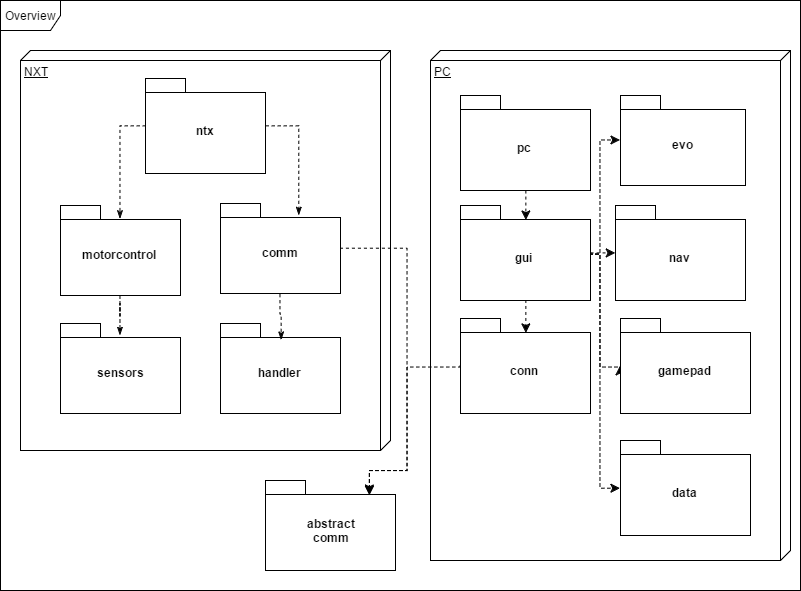
\includegraphics[width=\textwidth]{Overview.png}
    \caption{Übersicht der einzelnen Pakete in beiden Projekten.}
    \label{fig:Overview}
\end{figure}

\begin{figure}
	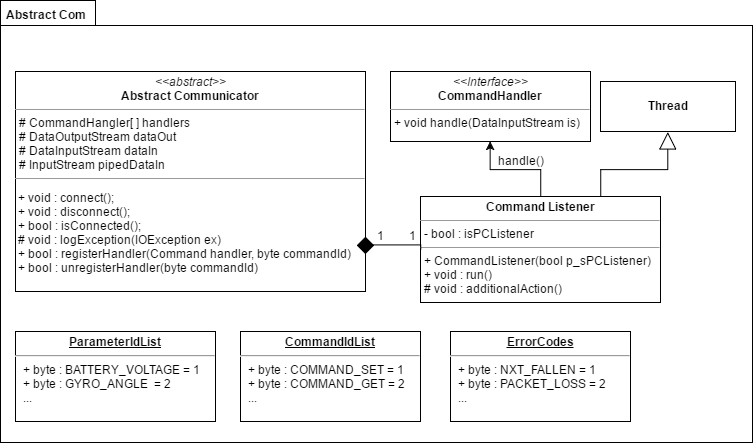
\includegraphics[width=\textwidth]{AbstractCom.png}
    \caption{Die abstrakte Kommunikationsklasse verbindet beide Projekte, indem sowohl das PC- als auch NXT-Projekt von dieser Klasse erben.}
    \label{fig:AbstractCom}
\end{figure}

\begin{figure}
	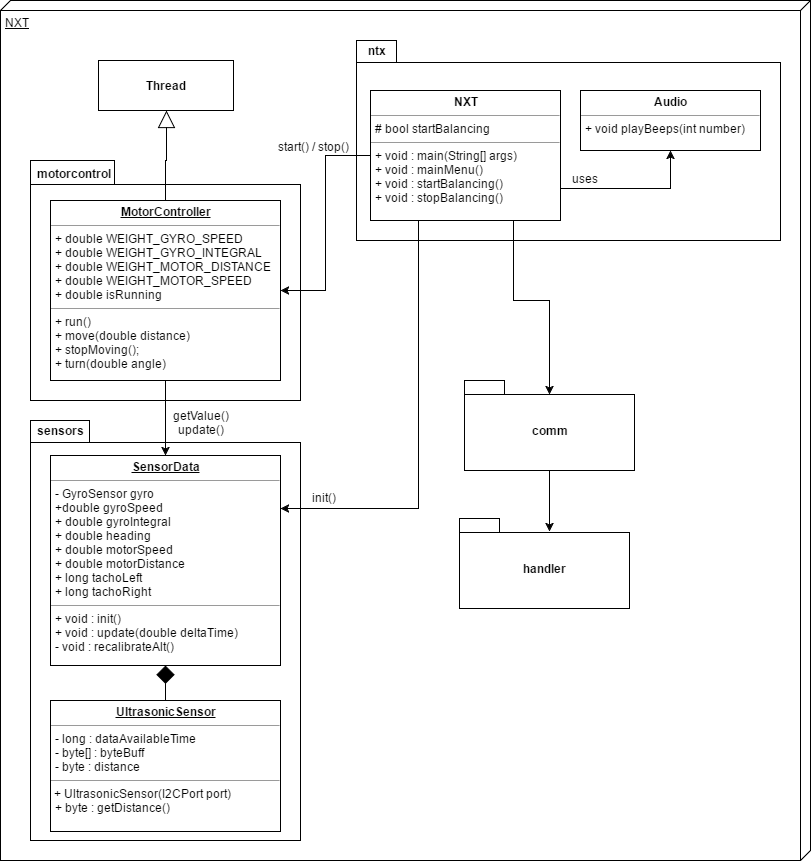
\includegraphics[width=\textwidth]{NXT.png}
    \caption{Der NXT besteht zur Hälfte aus dem MotorController in dem der Regler emuliert wird, dieser nutzt die Sensordaten, die in eigenen Klassen gehalten werden. Die andere Hälfte des NXT stellt die Kommunikationsklasse dar.}
    \label{fig:NXT}
\end{figure}

\begin{figure}
	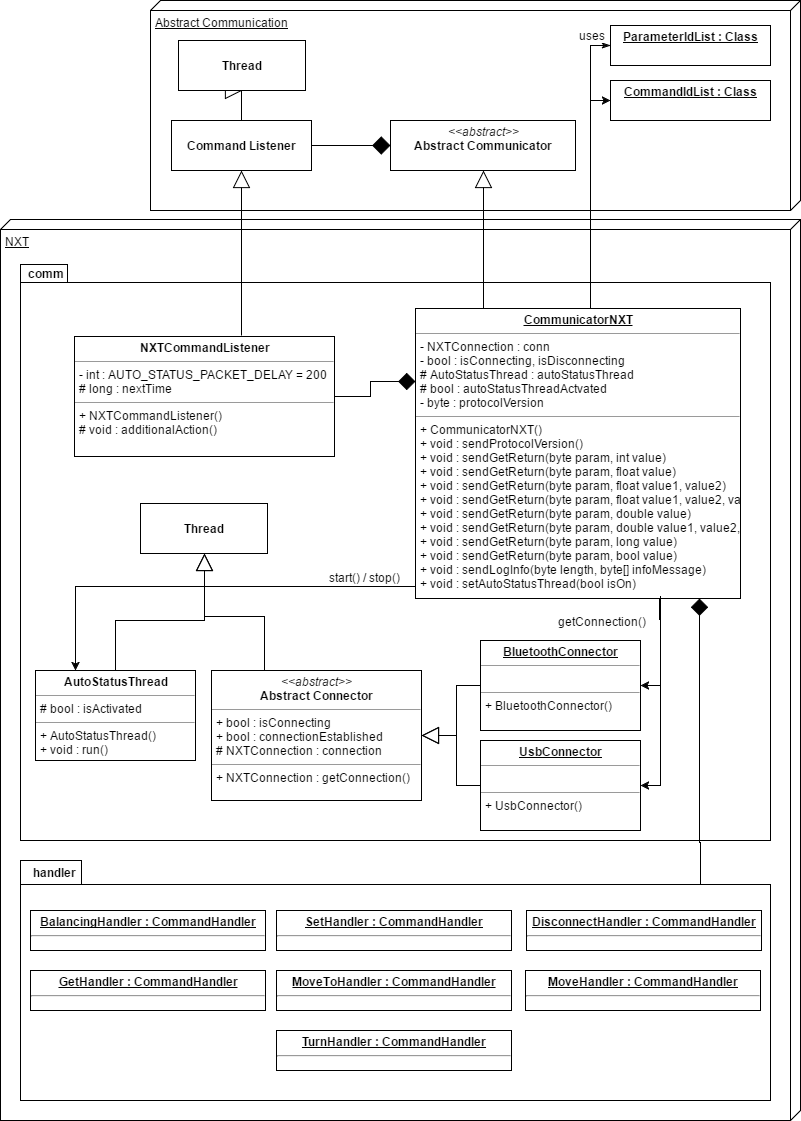
\includegraphics[width=\textwidth,height=0.9\textheight,keepaspectratio]{CommunicatorNXT.png}
    \caption{Die Kommunikationsklasse des NXT leitet sich vom abstrakten Kommunikator ab. Durch diesen können die Handler registriert werden und der NXT so auf Befehle reagieren.  }
    \label{fig:CommNXT}
\end{figure}

\begin{figure}
	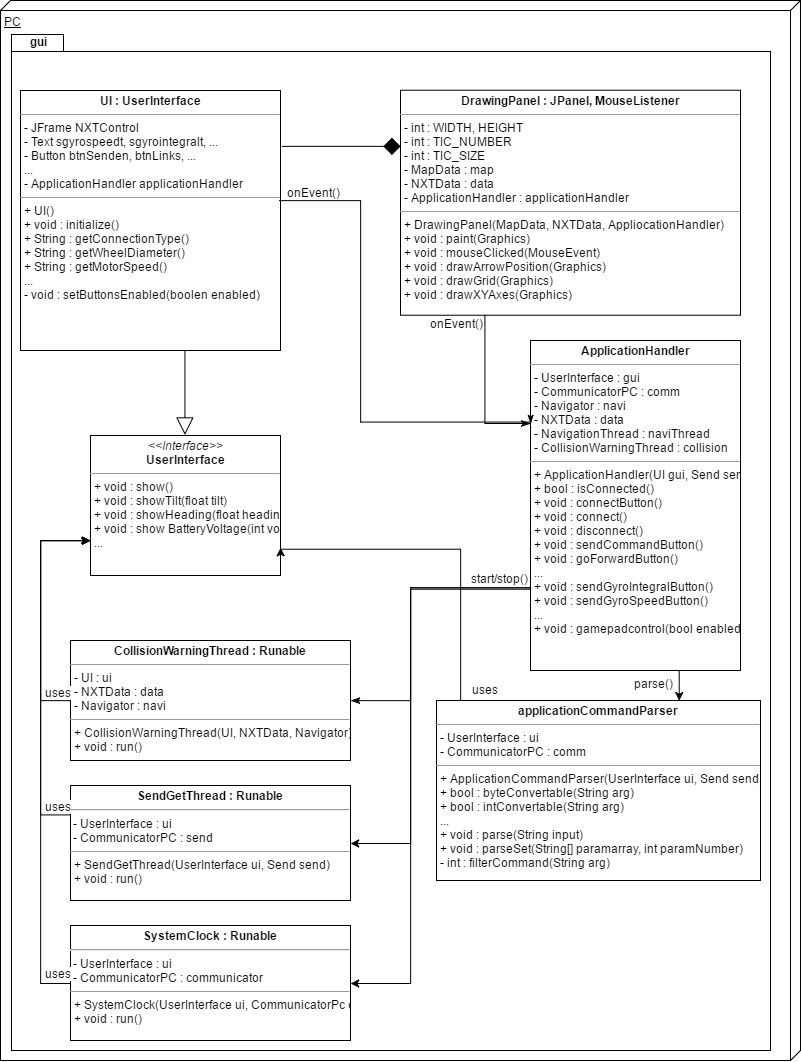
\includegraphics[width=\textwidth,height=0.85\textheight,keepaspectratio]{PCGui.png}
    \caption{Die GUI bildet das Zentrum der PC Architektur. von ihr aus werden alle anderen Komponenten erstellt und verwaltet. Durch die Verwendung des Interfaces und des Handlers wird die Anzeige von der Funktionalität entkoppelt.}
    \label{fig:GuiPC}
\end{figure}

\begin{figure}
	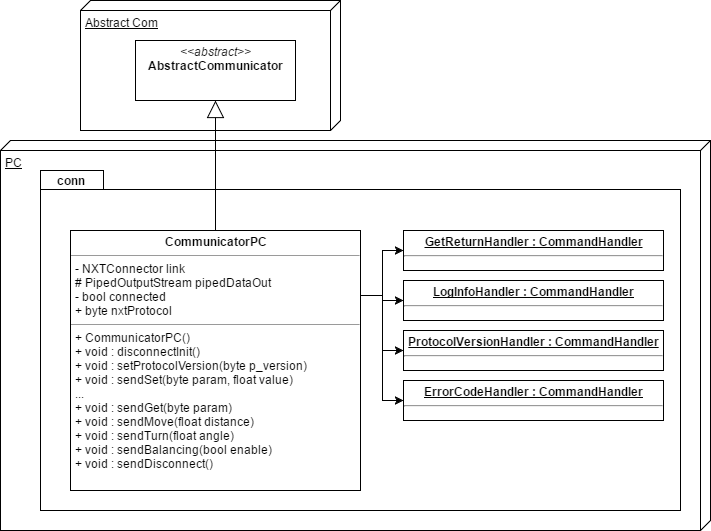
\includegraphics[width=\textwidth,height=\textheight,keepaspectratio]{ConnPC.png}
    \caption{Die Kommunikation auf der PC Seite wird vom CommunicatorPC durchgeführt. Dieser kann eine Verbindungsanfrage annehmen, durch diese Verbindung Nachrichten verschicken und auch Empfangen. Die Verarbeitung der Nachrichten übernehmen Handler, die zur Laufzeit registriert oder unregistriert werden können.}
    \label{fig:ConnPC}
\end{figure}

\begin{figure}
	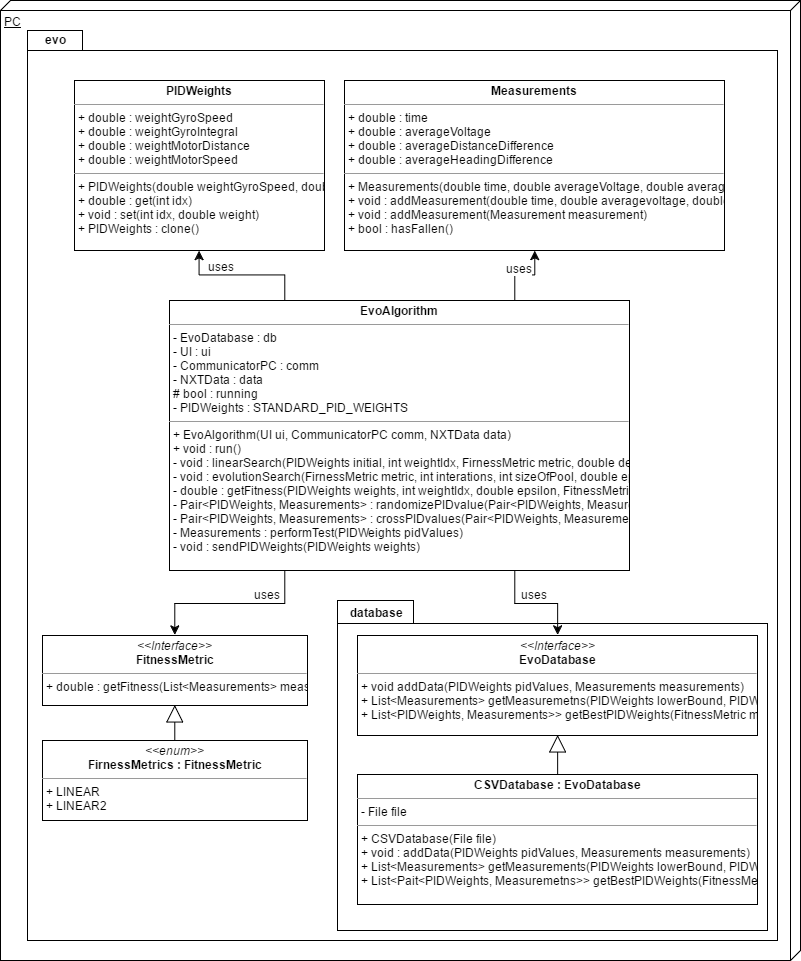
\includegraphics[width=\textwidth,height=\textheight,keepaspectratio]{evo.png}
    \caption{Das Evo Paket kapselt zwei Algorithmen zur Kalibrierung der PID Werte, sowie das Datenbanksystem. Das allgemeine Interface wurde durch eine CSV-Datenbank implementiert. Des Weiteren sind zwei Klassen für das Bündeln von Daten vorhanden, die PID-Gewichte und die Messungen verwalten. Die Metrik wird über ein Interface bereitgestellt, die Implementierung findet sich in einem Enum, das alle verfügbaren Metriken bündelt.}
    \label{fig:evo}
\end{figure}

\begin{figure}
	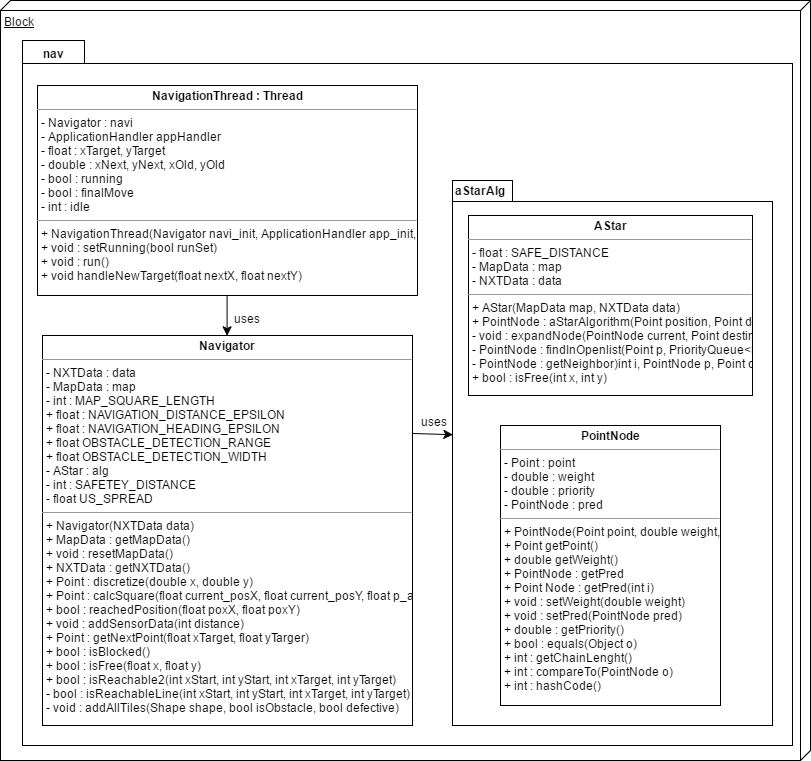
\includegraphics[width=\textwidth]{nav.png}
    \caption{Die Navigation wird in einem eigenem Thread ausgeführt, der den Navigator nutzt. Dieser benutzt die Datenklassen NXTData und MapData zur Bestimmung der Route und den A*-Algorithmus, der in einem eigenem Paket implementiert wurde.}
    \label{fig:nav}
\end{figure}

\begin{figure}
	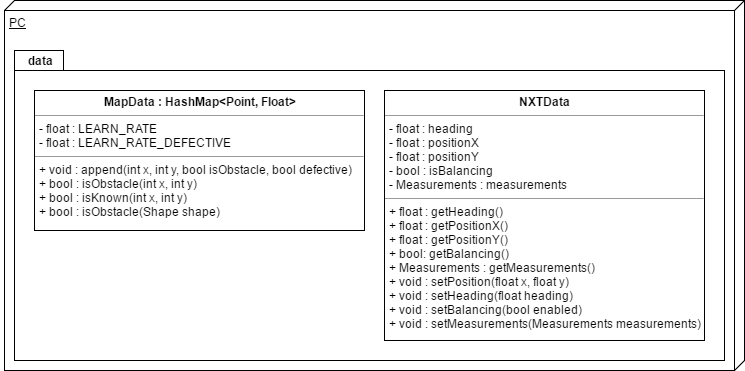
\includegraphics[width=\textwidth]{data.png}
    \caption{Die Daten der Karte wurden für einen effizienten Zugriff über eine HashMap implementiert. Die NXTData stellen eine virtuelle Abbildung des Zustands des NXT auf dem PC dar.}
    \label{fig:data}
\end{figure}

\begin{figure}
	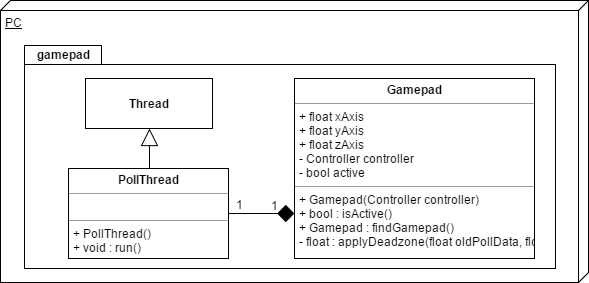
\includegraphics[width=\textwidth]{Gamepad.png}
    \caption{Die Gamepad-Klasse verwaltet externe Controller und sendet Steuerungsbefehle entsprechend der Eingabe an die Kommunikationsklasse weiter. Diese läuft in einem eigenem Thread.}
    \label{fig:Gamepad}
\end{figure}

\begin{figure}
	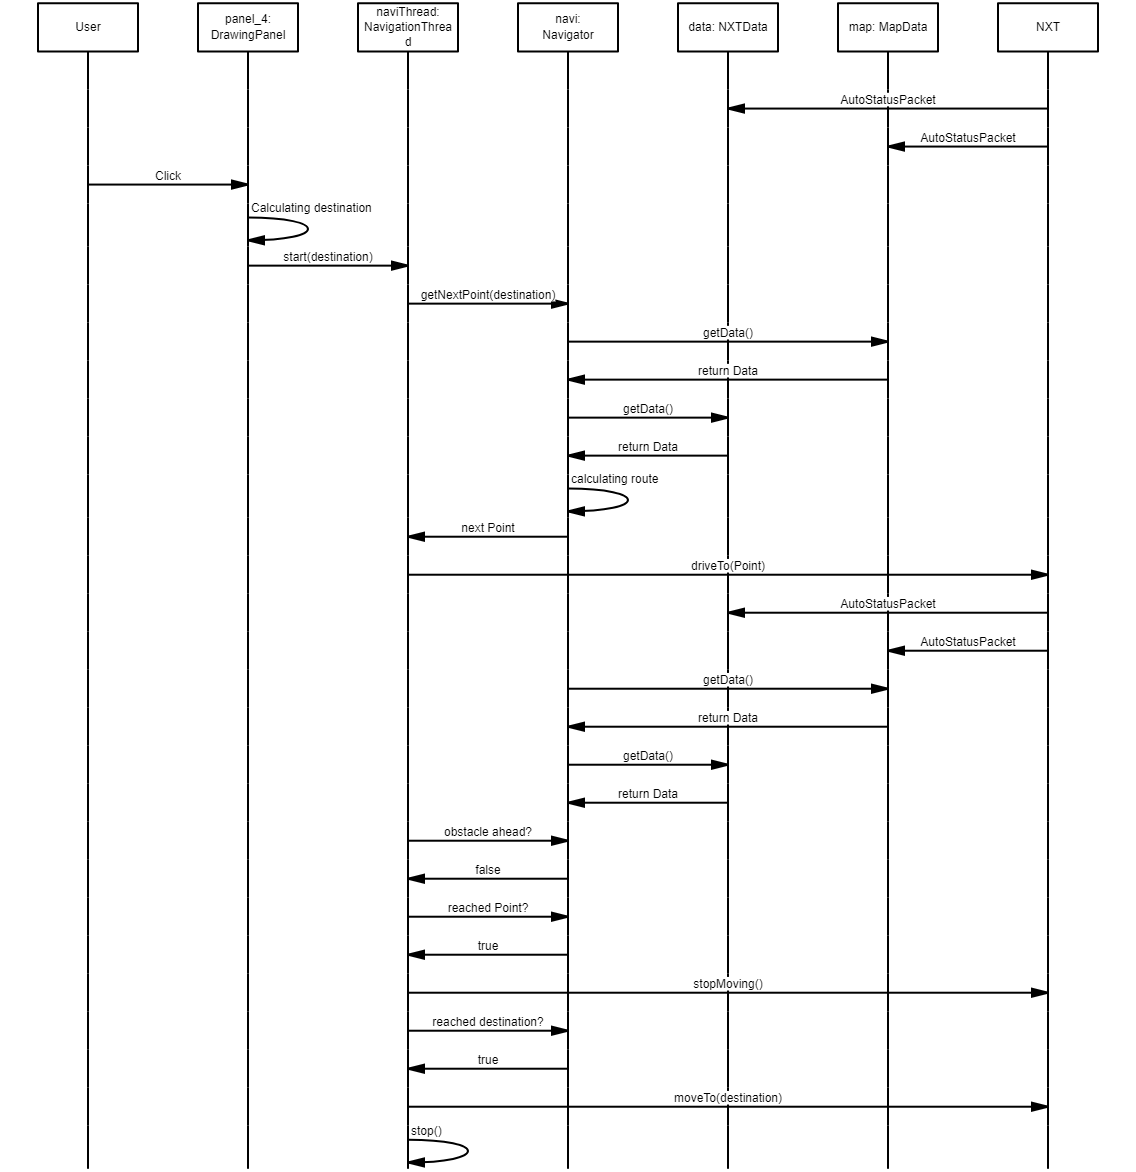
\includegraphics[width=\textwidth]{NavigationSequenceDiagram.png}
    \caption{Ein Beispiel des Ablaufs der Navigation mit Hindernisumfahrung}
    \label{fig:navSeqDia}
\end{figure}

\section{Kommunikationsprotokoll}

\begin{table}
	\caption{Command-Tabelle}
	\begin{tabular}{|l|l|l|l|}
		\hline
		\textbf{Command} & \textbf{CommandID} & \textbf{Richtung} & 		\textbf{Struktur} \\
         & \textbf{(0-255)} & & \\
		\hline
		Set & 1 & PC -> NXT & [commandID:byte][paramID:byte]\\
         & & & [value:varying] \\
		\hline
		Get & 2 & PC -> NXT & [commandID:byte][paramID:byte] \\
		\hline
		GetReturn & 3 & NXT -> PC & [commandID:byte][paramID:byte] \\
         & & & [value:varying] \\
		\hline
		Move & 4 & PC -> NXT & [commandID:byte][distance:float] \\
		\hline
		Turn & 5 & PC -> NXT & [commandID:byte][angle:float] \\
		\hline
		\textit{MoveTo <reserved>} & 6 & PC -> NXT & - \\
		\hline
		Balancing & 7 & PC -> NXT & [commandID:byte][enabled:boolean] \\
		\hline
		LogInfo & 8 & NXT -> PC & [commandID:byte][length:byte] \\
         & & & [message:byte[]] \\
		\hline
		ErrorCode & 9 & NXT -> PC & [commandID:byte][errorcode:byte] \\
		\hline
		Disconnect & 10 & PC -> NXT & [commandID:byte] \\
		\hline
		ProtocolVersion & 11 & NXT -> PC & [commandID:byte][protocolVersion:byte] \\
		\hline
	\end{tabular}
	\label{tab:cmdTable}
\end{table}

\begin{table}
	\caption{Parameter-Tabelle}
	\begin{tabular}{|l|l|l|l|l|l|}
		\hline
		\textbf{Parameter} & \textbf{ParamID} & \textbf{Get} & \textbf{Set} & \textbf{Typ} & \textbf{Einheit} \\
 		& \textbf{(0-255)} & & & & \\ 
		\hline
		BatteryVoltage & 1 & Ja & Nein & int & mV \\
		\hline
		GyroAngle & 2 & Ja & Nein & float & ° \\
		\hline
		TachoLeft & 3 & Ja & Nein & long & ° \\
		\hline
		TachoRight & 4 & Ja & Nein & long & ° \\
		\hline
		Heading & 5 & Ja & Ja & float & ° \\
		\hline
		Position & 6 & Ja & Ja & 2x float & cm \\
		\hline
		MovementSpeed & 7 & Ja & Nein & float & cm/s \\
		\hline
		StatusPacket & 8 & Ja & Nein & 4x float & - \\
		\hline
		AutoStatusPacket & 9 & Ja & Ja & boolean & - \\
		\hline
		PID-Gewichte <internal> & 21-30 & Ja & Ja & varying & - \\
		\hline
		\hline
		GyroSpeed & 21 & Ja & Ja & double & - \\
		\hline
		GyroIntegral & 22 & Ja & Ja & double & - \\
		\hline
		MotorDistance & 23 & Ja & Ja & double & - \\
		\hline
		MotorSpeed & 24 & Ja & Ja & double & - \\
		\hline
		Weightall & 128 & Ja & Ja & 4x double & - \\
		\hline
		ConstantRotation & 131 & Ja & Ja & float & °/s \\
		\hline
		ConstantSpeed & 132 & Ja & Ja & float & cm/s \\
		\hline
		WheelDiameter & 133 & Ja & Ja & float & cm \\
		\hline
		Track & 134 & Ja & Ja & float & cm \\
		\hline
		UltraSensor & 135 & Nein & Nein & int & cm \\
		\hline
		CollectTestData & 140 & Nein & Ja & boolean & - \\
		\hline
		Measurements & 141 & Nein & Nein & 4x double & - \\
		\hline
	\end{tabular}
	\label{tab:paramTable}
\end{table}

\end{document}